\documentclass[11pt]{article}
\usepackage{setspace}
\setstretch{1}
\usepackage{amsmath,amssymb, amsthm}
\usepackage{graphicx}
\usepackage{bm}
\usepackage[hang, flushmargin]{footmisc}
\usepackage[colorlinks=true]{hyperref}
\usepackage[nameinlink]{cleveref}
\usepackage{footnotebackref}
\usepackage{url}
\usepackage{listings}
\usepackage[most]{tcolorbox}
\usepackage{inconsolata}
\usepackage[papersize={8.5in,11in}, margin=1in]{geometry}
\usepackage{float}
\usepackage{caption}
\usepackage{esint}
\usepackage{url}
\usepackage{enumitem}
\usepackage{subfig}
\usepackage{wasysym}
\newcommand{\ilc}{\texttt}
\newcommand{\p}{\partial}
\usepackage{etoolbox}
\usepackage{algorithm}
\usepackage{changepage}
% \usepackage{algorithmic}
\usepackage[noend]{algpseudocode}
\usepackage{tikz}


\usetikzlibrary{matrix,positioning,arrows.meta,arrows}
\patchcmd{\thebibliography}{\section*{\refname}}{}{}{}
% \PassOptionsToPackage{hyphens}{url}\usepackage{hyperref}

\providecommand{\myceil}[1]{\left \lceil #1 \right \rceil }
\providecommand{\myfloor}[1]{\left \lfloor #1 \right \rfloor }
\providecommand{\qbm}[1]{\begin{bmatrix} #1 \end{bmatrix}}
\providecommand{\qpm}[1]{\begin{pmatrix} #1 \end{pmatrix}}
\providecommand{\norm}[1]{\left\lVert #1 \right\rVert}
\providecommand{\len}[1]{\left| #1 \right|}
\newcommand{\cmark}{\ding{51}}%
\newcommand{\xmark}{\ding{55}}%

\definecolor{dkgreen}{rgb}{0,0.6,0}
\definecolor{gray}{rgb}{0.5,0.5,0.5}
\definecolor{mauve}{rgb}{0.58,0,0.82}

\lstset{frame=tb,
  language=Python,
  aboveskip=3mm,
  belowskip=3mm,
  showstringspaces=false,
  columns=flexible,
  basicstyle={\small\ttfamily},
  numbers=none,
  numberstyle=\tiny\color{gray},
  keywordstyle=\color{blue},
  commentstyle=\color{dkgreen},
  stringstyle=\color{mauve},
  breaklines=true,
  breakatwhitespace=true,
  tabsize=3
}

\begin{document}


\title{\textbf{CSDS 491: Assignment 4}}

\author{Shaochen (Henry) ZHONG, \ilc{sxz517@case.edu}}

\date{Due and submitted on 04/21/2021 \\ Spring 2021, Dr. Lewicki}
\maketitle

\section*{E1. Multivariate Gaussians}

Please refer to \ilc{A4/code/e1.py} for the code implmentations of below plots.

\subsection*{1.1.}

For 2D multivariate normal we have $\Sigma = \qbm{\sigma_{xx} & \sigma_{xy} \\ \sigma_{yx} & \sigma_{yy}}$. Note:

\begin{itemize}
    \item For $x$ and $y$ to be uncorrelated, we have $\sigma_{xy} = \sigma_{yx} = 0$. For demo, we have $\mathcal N(\mu = \qbm{0 \\ 0}, \Sigma = \qbm{1 & 0 \\ 0 & 1})$.
    \item For $x$ and $y$ to be uncorrelated, we have $\sigma_{xy} = \sigma_{yx} > 0$. For demo, we have $\mathcal N(\mu = \qbm{0.5 \\ 0.5}, \Sigma = \qbm{1 & 0.9 \\ 0.9 & 1})$.
    \item For $x$ and $y$ to be anti-correlated, we have $\sigma_{xy} = \sigma_{yx} < 0$. For demo, we have $\mathcal N(\mu = \qbm{0.7 \\ 0.7}, \Sigma = \qbm{1 & -0.9 \\ -0.9 & 1})$.
\end{itemize}

\begin{figure}[H]
\minipage{0.3\textwidth}
  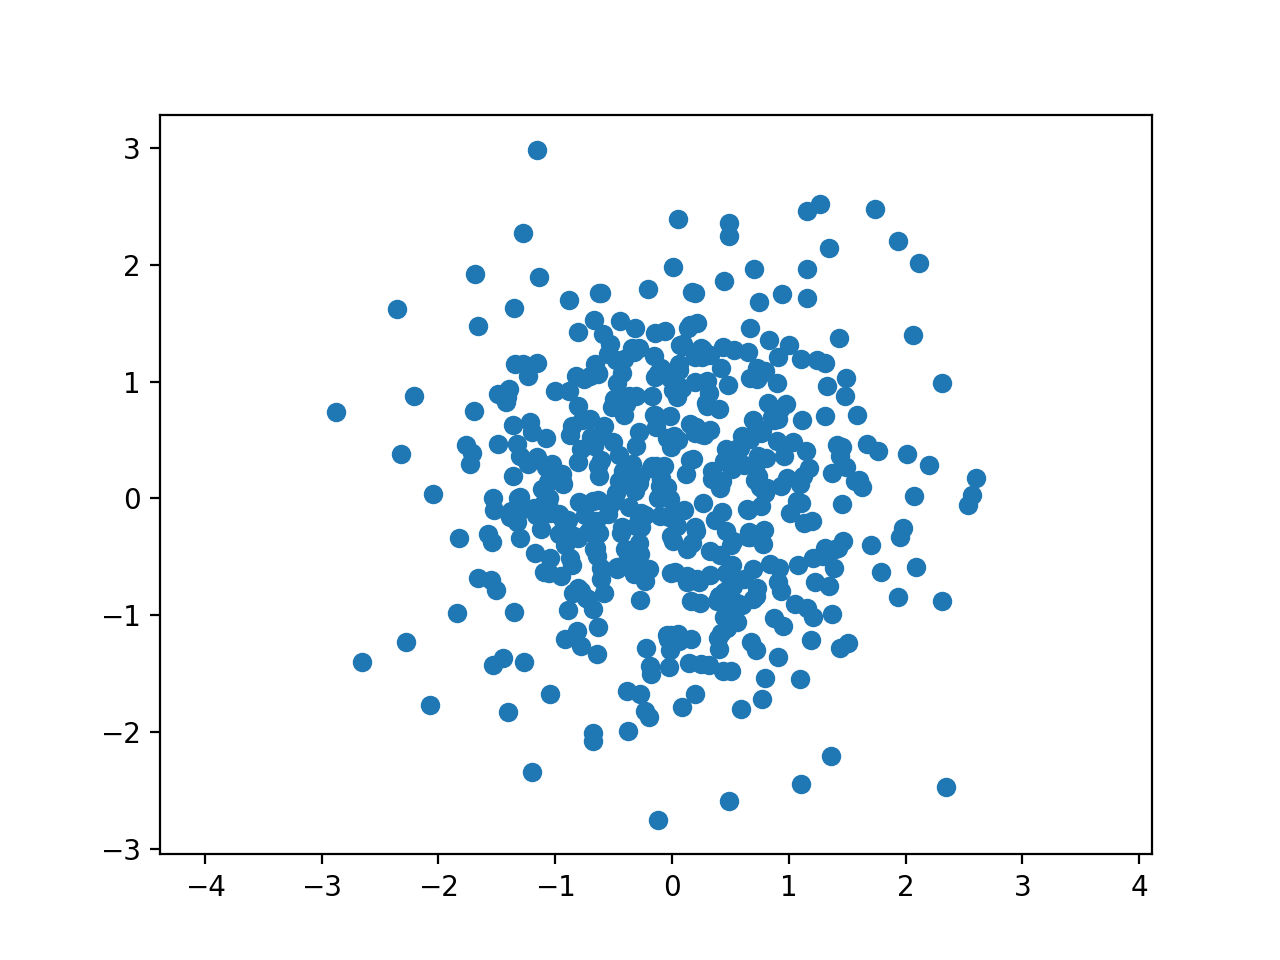
\includegraphics[width=\linewidth]{{fig/e1.1_1}.png}
  \caption*{Uncorrelated}
\endminipage\hfill
\minipage{0.3\textwidth}
    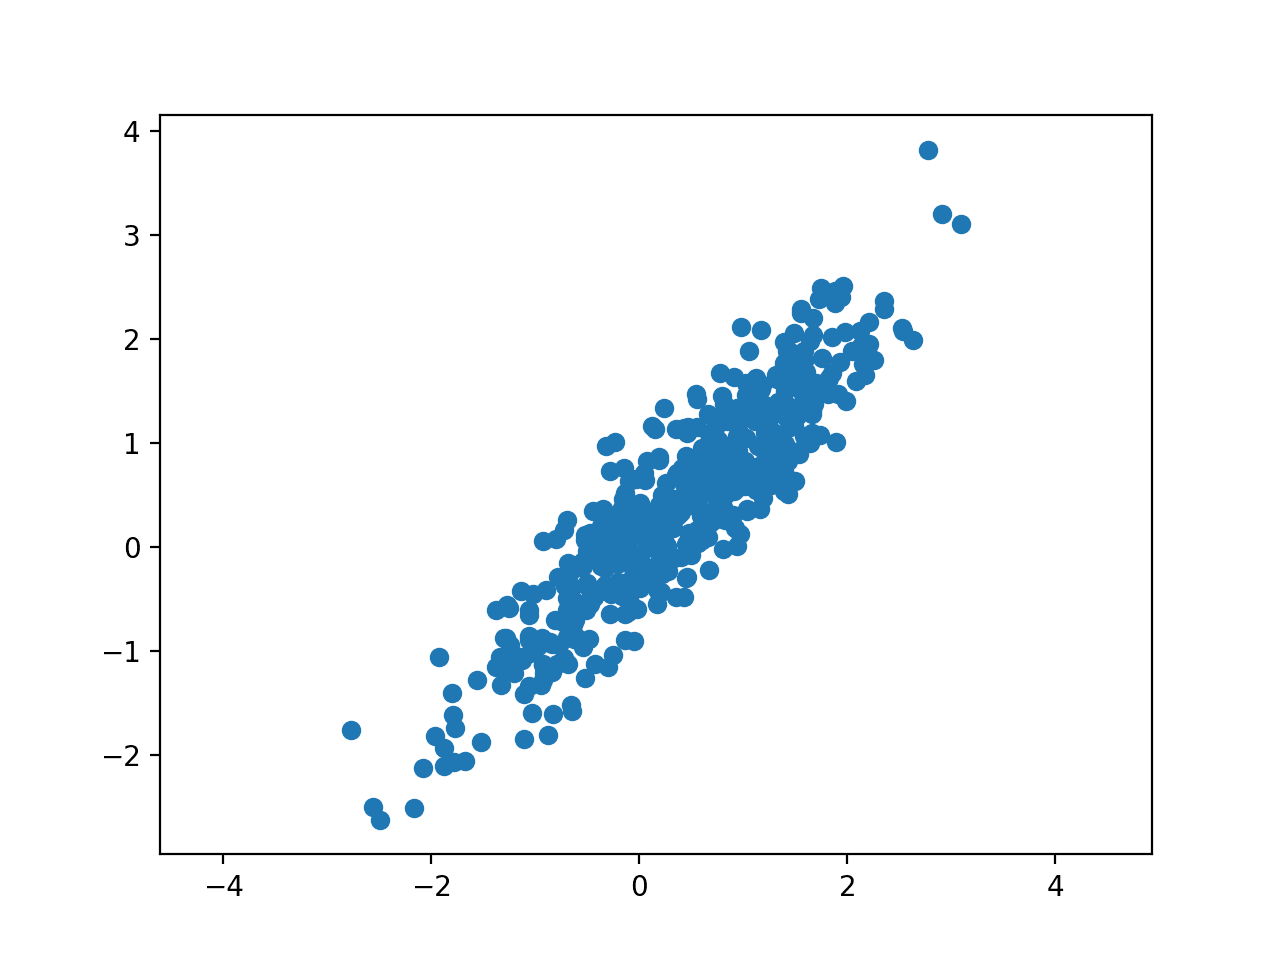
\includegraphics[width=\linewidth]{{fig/e1.1_2}.png}
    \caption*{Correlated}
\endminipage\hfill
\minipage{0.3\textwidth}
    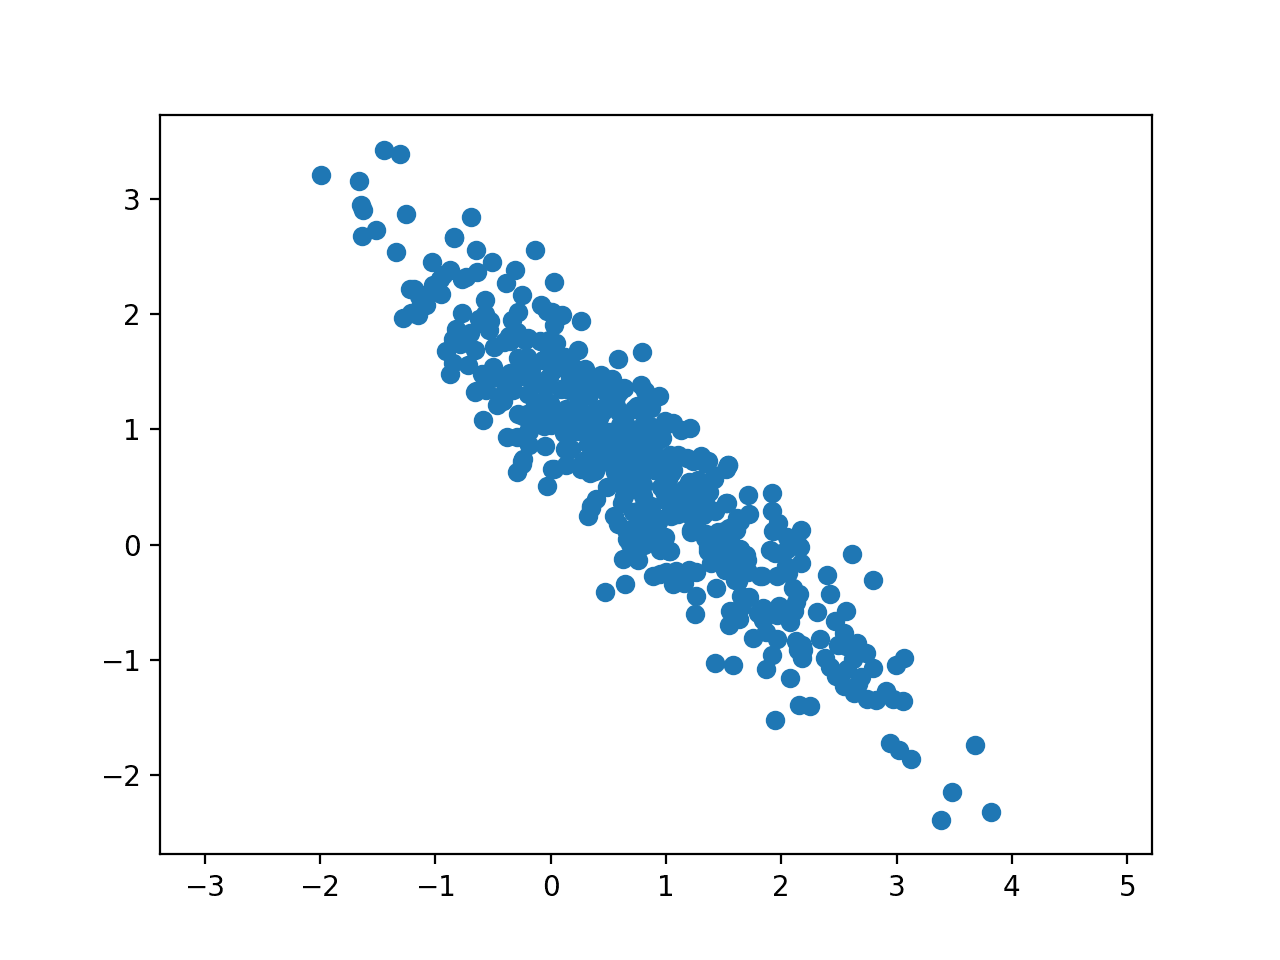
\includegraphics[width=\linewidth]{{fig/e1.1_3}.png}
    \caption*{Anti-correlated}
\endminipage
\end{figure}


\subsection*{1.2.}

Assuming the same $\mu$ and $\Sigma$ setup in \textbf{Exercise 1.1}, we have the $1-, 2-, 3-\sigma$ countour plots being (note eigenvectors are scaled \ilc{4x} for visual purposes):


\begin{figure}[H]
\minipage{0.3\textwidth}
  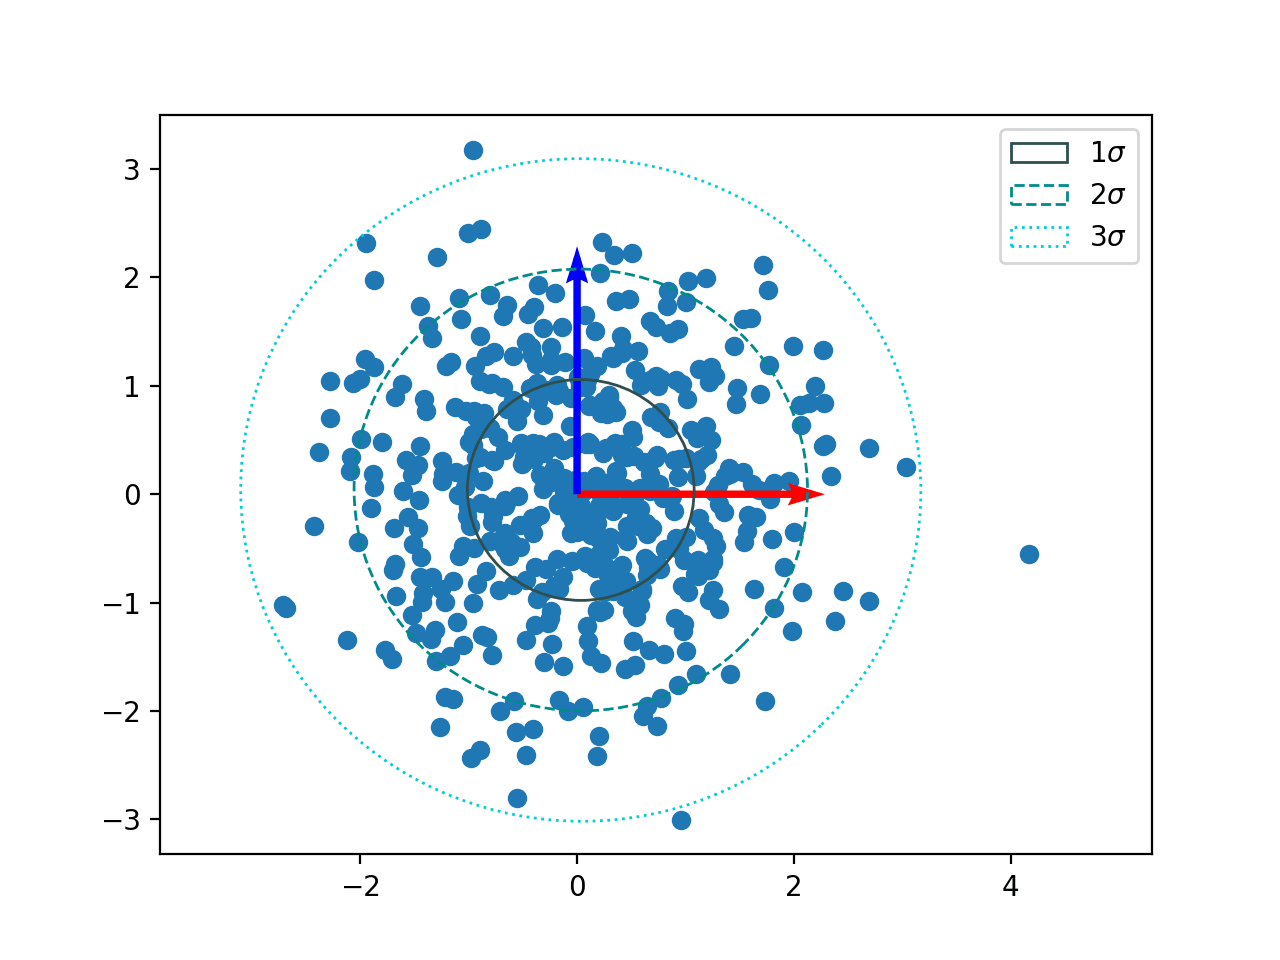
\includegraphics[width=\linewidth]{{fig/e1.2_1}.png}
  \caption*{Uncorrelated}
\endminipage\hfill
\minipage{0.3\textwidth}
    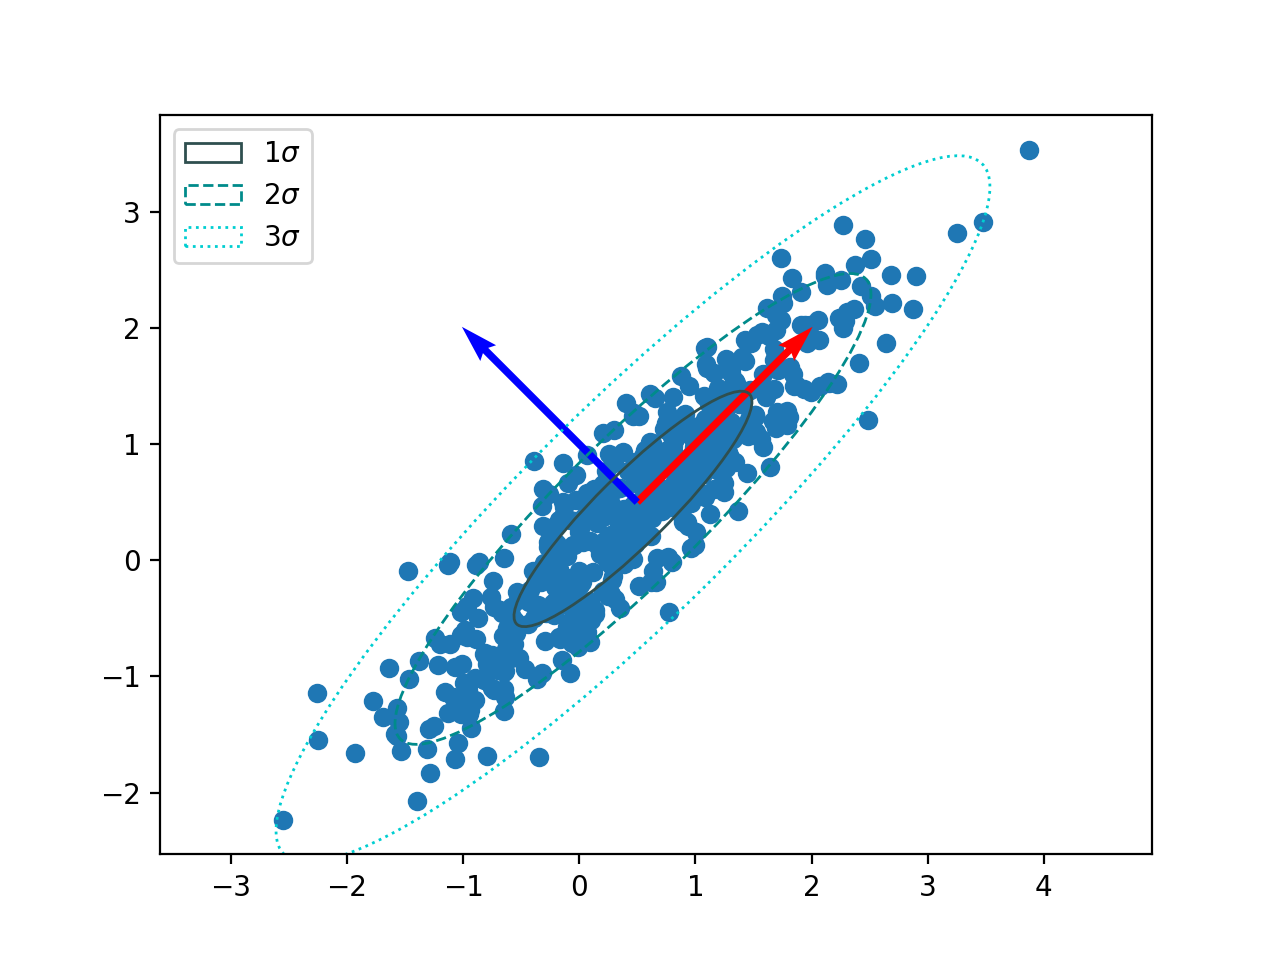
\includegraphics[width=\linewidth]{{fig/e1.2_2}.png}
    \caption*{Correlated}
\endminipage\hfill
\minipage{0.3\textwidth}
    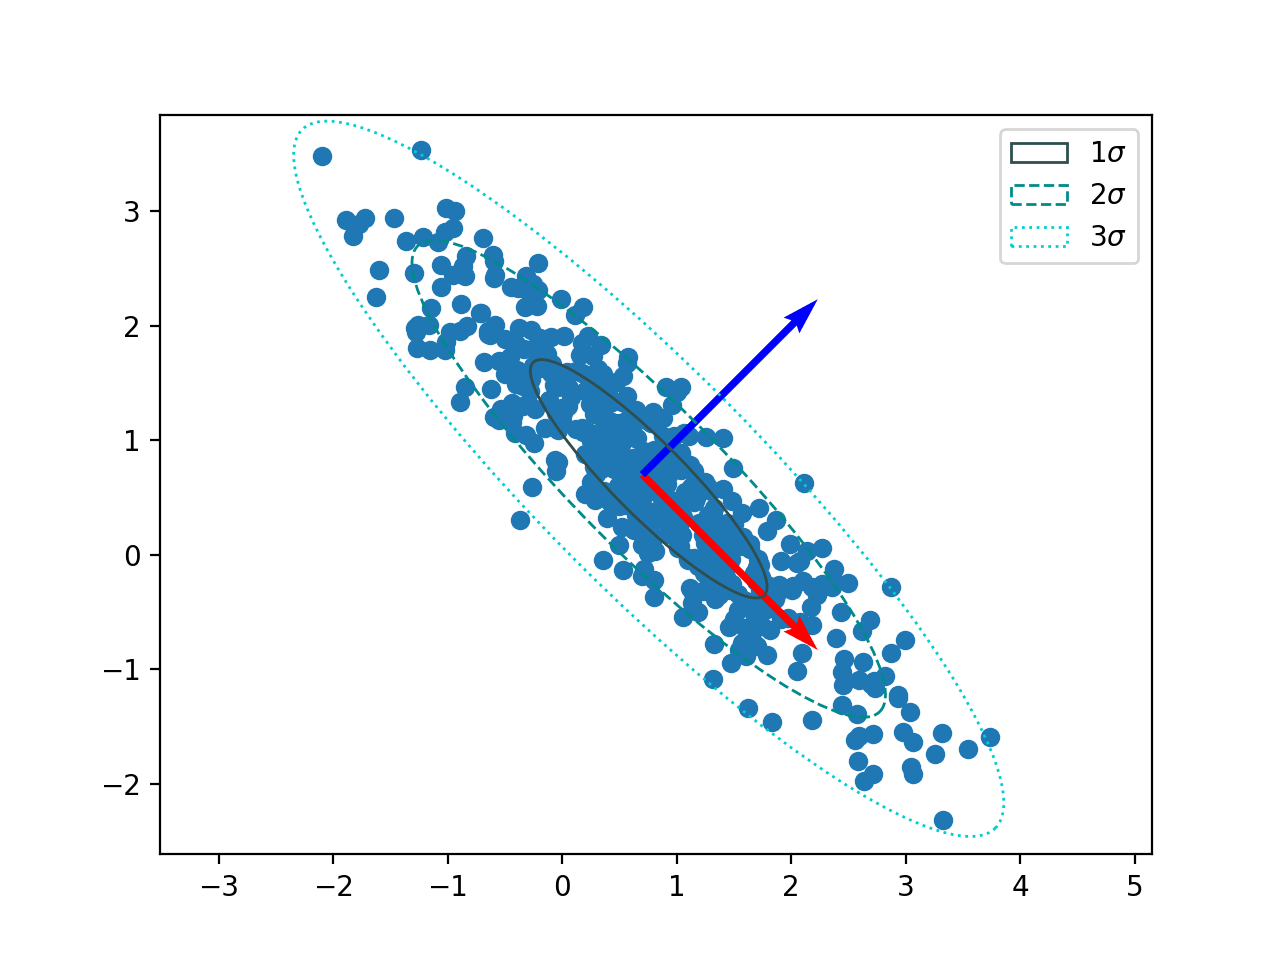
\includegraphics[width=\linewidth]{{fig/e1.2_3}.png}
    \caption*{Anti-correlated}
\endminipage
\end{figure}



\section*{E2. Linear Gaussian Models}

\subsection*{2.1.}
% https://math.stackexchange.com/questions/60911/multivariate-normal-difference-distribution
% https://stats.stackexchange.com/questions/9879/addition-of-multivariate-gaussians

Known the characteristic functions of $x$ and $z$ is:

\begin{align*}
    \phi_x(u) &= \exp(i u^T \mu_x - \frac{1}{2} u^T \Sigma_x u) \\
    \phi_z(u) &= \exp(i u^T \mu_z - \frac{1}{2} u^T \Sigma_z u)
\end{align*}

Since $x$ and $z$ are independent, their sum will still conform to the normal distribution. We may confirm it by analysing the characteristic functions of $x + z$, which is $\phi_{x + z}(u) = E(e^{it(x + z)}) = E(e^{itx}) \cdot E(e^{itz}) = \phi_{x}(u) \phi_{z}(u)$, then we have:

\begin{align*}
    \phi_{x + z}(u) &= \phi_{x}(u) \phi_{z}(u) = \exp(i u^T \mu_x - \frac{1}{2} u^T \Sigma_x u) \cdot \exp(i u^T \mu_z - \frac{1}{2} u^T \Sigma_z u) \\
    &= \exp(i u^T (\mu_x + \mu_z) - \frac{1}{2} u^T (\Sigma_x + \Sigma_z) u) \\
    \Longrightarrow \phi_y(u) &= \exp(i u^T \mu_y - \frac{1}{2} u^T \Sigma_y u)
\end{align*}

Thus, we have $p(y) = \mathcal N(\mu_x+\mu_z,\Sigma_x+\Sigma_z)$.


\subsection*{2.2.}

% https://stats.stackexchange.com/questions/30588/deriving-the-conditional-distributions-of-a-multivariate-normal-distribution
% http://www.math.chalmers.se/~rootzen/highdimensional/SSP4SE-appA.pdf
% http://users.stat.umn.edu/~helwig/notes/norm-Notes.pdf
% https://www.coursera.org/lecture/linear-models-2/normal-conditional-distributions-LiHmE

For clarity, we let $p(x, y) = \mathcal N(\mu, \Sigma)$, where:

\begin{align*}
    \mu &= \qbm{\mu_x \\ \mu_y} \\
    \Sigma &= \qbm{\Sigma_{xx} & \Sigma_{xy} \\ \Sigma_{yx} & \Sigma_{yy}}
\end{align*}

Note each of $\Sigma{ab}$ is a matrix of $a \times b$.

We further know that there must be $p(y \mid x) = \mathcal N(\overline{\mu}, \overline{\Sigma})$, where:

\begin{align*}
    \overline{\mu} &= \mu_y + \Sigma_{yx} \Sigma_{xx}^{-1} (x - \mu_x) \\
    \overline{\Sigma} &= \Sigma_{yy} - \Sigma_{yx} \Sigma_{xx}^{-1}\sigma{yx}
\end{align*}

I don't know if we are expected to show the proof, but here's a trick that can do it rather quickly. Assume $z = y + Ax$ (not to be confused with the $z$ in \textbf{Question 2.1}) with $A = -\Sigma_{yx} \Sigma_{xx}^{-1}$, we have:

\begin{align*}
    cov(z, x) &= cov(y + Ax, x) = cov(y, x) + A \cov(x, x) \\
    &= \Sigma_{yx} + (-\Sigma_{yx} \Sigma_{xx}^-1) \Sigma_{xx} \\
    &\text{Now to deduce $E(y \mid x)$} \\
    \Rightarrow &\begin{cases}
        E(z | x) &= E(z) = E(y + Ax) = \mu_y + A \mu_x = \mu_y -\Sigma_{yx} \Sigma_{xx}^{-1} \mu_x \\
        E(z | x) &= E(y + Ax \mid x) = E(y \mid x) + A E(x \mid x) \\
    \end{cases} \\
    \Longrightarrow E(y \mid x) &= E(z | x) - A E(x \mid x) = \mu_y -\Sigma_{yx} \Sigma_{xx}^{-1} \mu_x - (-\Sigma_{yx} \Sigma_{xx}^{-1}) x \\
    &= \mu_y + \Sigma_{yx} \Sigma_{xx}^{-1} (x - \mu_x) = \overline{\mu}
\end{align*}


Similarily, we may find out $\overline{\Sigma}$ as (note that $cov(x, y) = cov(y, x)$):


\begin{align*}
    var(y \mid x) &= var(z) = var(y + Ax) \\
    &= var(y) + A var(x) A' + A cov(y, x) + cov(x, y) A' \\
    &= \Sigma_{yy} + \Sigma_{yx} \Sigma_{xx}^{-1} \Sigma_{xx} \Sigma_{xx}^{-1} \Sigma_{xy} - \Sigma_{yx} \Sigma_{xx}^{-1} \Sigma_{yx} - \Sigma_{yx} \Sigma_{xx}^{-1} \Sigma_{xy} \\
    &= \Sigma_{yy} + \Sigma_{yx} \Sigma_{xx}^{-1} \Sigma_{xy} - 2 \Sigma_{yx} \Sigma_{xx}^{-1} \Sigma_{xy} \\
    \Longrightarrow \overline{\Sigma}&= \Sigma_{yy} - \Sigma_{yx} \Sigma_{xx}^{-1} \Sigma_{xy}
\end{align*}


As know from \textbf{Exercise 2.1} that $p(y) = \mathcal N(\mu_x+\mu_z,\Sigma_x+\Sigma_z)$ and $p(x) = \mathcal N(\mu_x, \Sigma_x)$, we have $p(y \mid x) = \mathcal N(\overline{\mu}, \overline{\Sigma})$, where:

\begin{align*}
    \overline{\mu} &= \mu_y + \Sigma_{yx} \Sigma_{xx}^{-1} (x - \mu_x) = \mu_x + \mu_z + \Sigma_{yx} \Sigma_{xx}^{-1} (x - \mu_x) \\
    \overline{\Sigma} &=  \Sigma_{yy} - \Sigma_{yx} \Sigma_{xx}^{-1} \Sigma_{xy} = \Sigma_{x} + \Sigma_{z} -\Sigma_{yx} \Sigma_{xx}^{-1} \Sigma_{xy}
\end{align*}

\subsection*{2.3.}

According to \textbf{Exercise 2.1}, for $y = x + z$, we have $y \sim \mathcal N(\mu_x+\mu_z,\Sigma_x+\Sigma_z)$. For the ease of demo, let $\sigma_x = 3$ and $\sigma_z = 4$ so that we may have the nice $\sigma_x^2 + \sigma_z^2 = \sigma_y^2 \Longleftrightarrow 3^2 + 4^2 = 5^2$ relationship. In such case, we may have:




\begin{align*}
    p(x) &= \mathcal N(\mu_x = 0, \Sigma_x = 3^2) \\
    p(y) &= \mathcal N(\mu_y = 1, \Sigma_y = 4^2) \\
    p(z) &= \mathcal N(\mu_x+\mu_z,\Sigma_x+\Sigma_z) = \mathcal N(\mu_x = 1, \Sigma_x = 5^2)
\end{align*}

The plots will look like:


\begin{figure}[H]
    \centering
    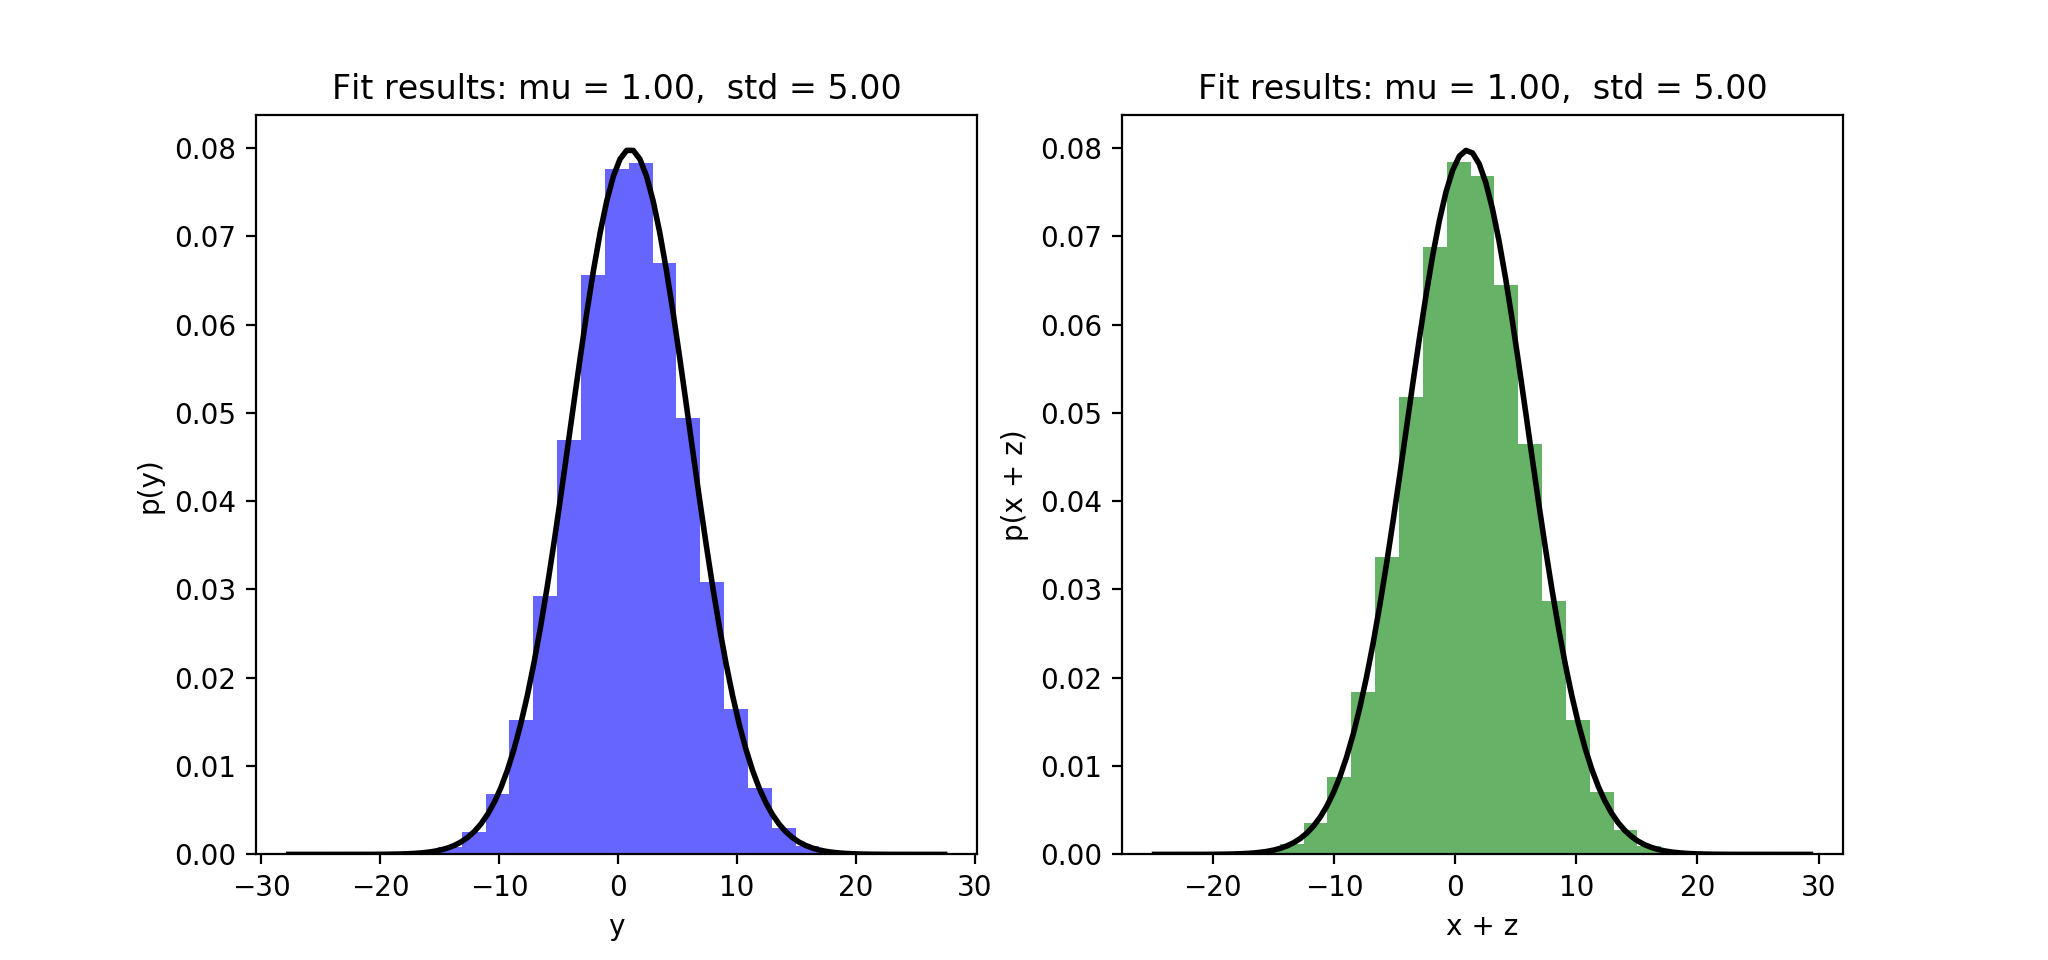
\includegraphics[width=1\linewidth]{{fig/e2.3}.png}
\end{figure}

We may tell these two plots are close resemblance of one and another by inspecting the shape of graph and the parameter of the fitted curve (showed as title of each plot).\newline

Please refer to \ilc{code/p2.py} for the code implementation.

\section*{E3. dimensionality Reduction and PCA}

\subsection*{3.1.}

The dataset I used in this exercise is the UCI Machine Learning \textit{Glass Classification} dataset I obtained from \href{https://www.kaggle.com/uciml/glass}{Kaggle}.

\begin{lstlisting}
        RI     Na    Mg    Al     Si     K    Ca   Ba   Fe  Type
0  1.52101  13.64  4.49  1.10  71.78  0.06  8.75  0.0  0.0     1
1  1.51761  13.89  3.60  1.36  72.73  0.48  7.83  0.0  0.0     1
2  1.51618  13.53  3.55  1.54  72.99  0.39  7.78  0.0  0.0     1
3  1.51766  13.21  3.69  1.29  72.61  0.57  8.22  0.0  0.0     1
4  1.51742  13.27  3.62  1.24  73.08  0.55  8.07  0.0  0.0     1
...
(214, 10)
\end{lstlisting}

As showned above, it is a dataset of 214 sample, each with 9 attributes, and each sample has a label that belong to 7 of the potential glass types. The attributes is rather straightforward, with \ilc{RI} being refractive index, and all the others are  chemistry elements measured by weight percent in corresponding oxide (e.g. \ilc{Na} is Sodium, \ilc{Mg} is Magnesium, etc). The output labels are something among the lines of \ilc{container}, \ilc{tableware}, and \ilc{headlamps}.

I opted to use this dataset as this is one of the few lightweight datasets with continues variables that I may find, and it has more than 6 dimensions. It probably doesn't make much sense to illustrate the dataset further, but the Kaggle page I linked above has some distribution plots for each element -- if you are interested. One thing to note about this dataset is, due to its lightweight, the dataset is really unbalanced as it has \ilc{70} samples on \ilc{Type 1}, \ilc{76} samples on \ilc{Type 1}, but only \ilc{17, 13, 9, 29} samples on \ilc{Type 3, 5, 6, 7} respectively (yes, \ilc{Type 4: vehicle} is entirely missing).

\subsection*{3.2.}

As we can't nicely plot 9-dimensional data. The first three eigenvalues and their corresponding eigenvectors are:

\begin{lstlisting}
3.00200916e+00 1.65917340e+00 6.79576475e-01

[-9.28126899e-04  1.52290883e-03 -1.37689385e-03  3.10643441e-04
-7.12950233e-04 -1.82174928e-03 -3.32594524e-04 -4.12235755e-03 9.99986948e-01]
[-1.72248332e-02 -3.98797552e-01 -6.54934730e-01 -3.46599960e-01
3.98381798e-01  1.55680962e-02 -3.76900981e-02 -3.62242832e-01 -1.39622177e-03]
[ 7.23534913e-01  5.43050989e-01 -1.31198879e-01 -9.86931157e-02
-7.68490459e-02  4.77602532e-02 -7.49534298e-02 -3.75274748e-01 -1.84522571e-03]
\end{lstlisting}

First we may confirm that the eigenvalues are indeed sorted in decreasing order, suggesting an eigenvalue with smaller index implies greater squared sum of variances and therefore accounts for higher percentage of variation.

We may also confirm that these eigenvectors are indeed 9-dimensional as expected, and they are orthognal to eachother as the inner products between them yield 0:

\begin{lstlisting}
<v_1, v_2> = 4.336808689942018e-19
<v_2, v_3> = -5.551115123125783e-17
<v_1, v_3> = -4.336808689942018e-19
\end{lstlisting}
(There are not exactly zero due to datatype accuracy problem, but with at least $10^{-17}$ they are close enough to zero.)

Note the magnitutde of the entries of each eigenvalues are similar, with the exception that the first eigenvector shows greater value on element \ilc{Fe}, the first eigenvector shows lesser value on element \ilc{Mg}, and the third eigenvector shows greater value on \ilc{RI} (the reflective index) -- suggesting that the classification of glass samples might be postively correlated to \ilc{Fe} and \ilc{RI}, and negatively correlated to \ilc{Mg}. In terms of co-vary between eigenvectors, it is hard to tell if there is much consistency.

\subsection*{3.3.}

\begin{figure}[H]
    \centering
    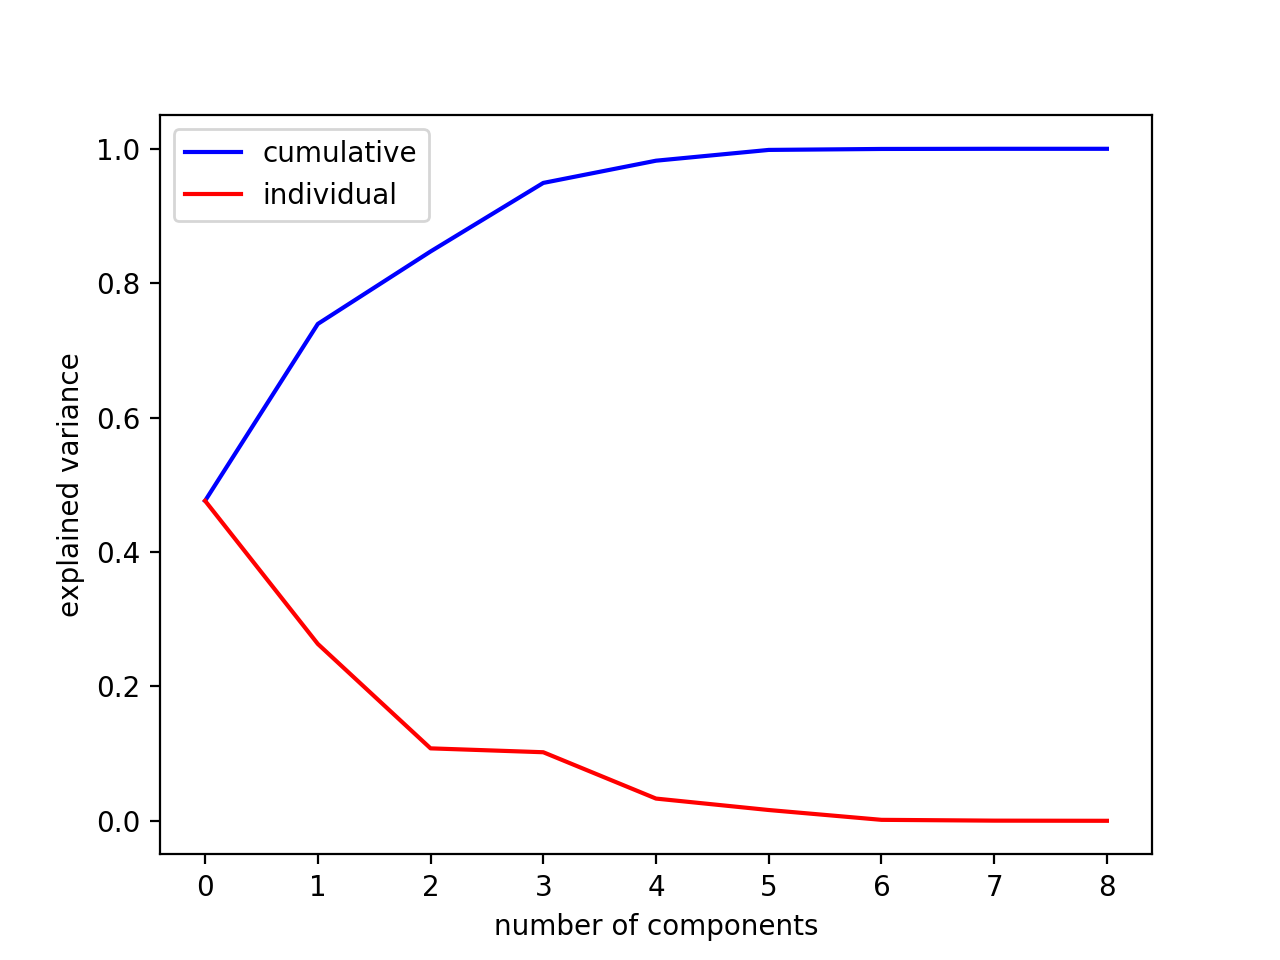
\includegraphics[width=0.5\linewidth]{{fig/e3.3}.png}
\end{figure}

The \textcolor{red}{red} line represents the percentage of variation that particular principle component accounts for. In this case, as we are ploting with respect to the decreasing order of eigenvalues, each principle component accountss for less variation than the previous one. Reversely, the \textcolor{blue}{blue}, whic represents the cumulative variance, is increasing as we add in more principle components -- and when we have all principle components (which is the dimension of the attributes or number of samples, in this case it is the former) considered, the cummulative explained variance reaches 1.

\subsection*{3.4.}

By reducing the dataset to 2 dimensions (\ilc{PC1, PC2}) -- meaning that these two eigenvectors has the two largest eigenvalues, suggesting the range of data projection are more distinguishiable on these two eigenvectors and therefore they contain most information -- we may have the following plot. Note the data were standardized with respect to their mean in this plot and throughout the PCA process, so that we won't have one catagory of data dominating all the others:

\begin{figure}[H]
    \centering
    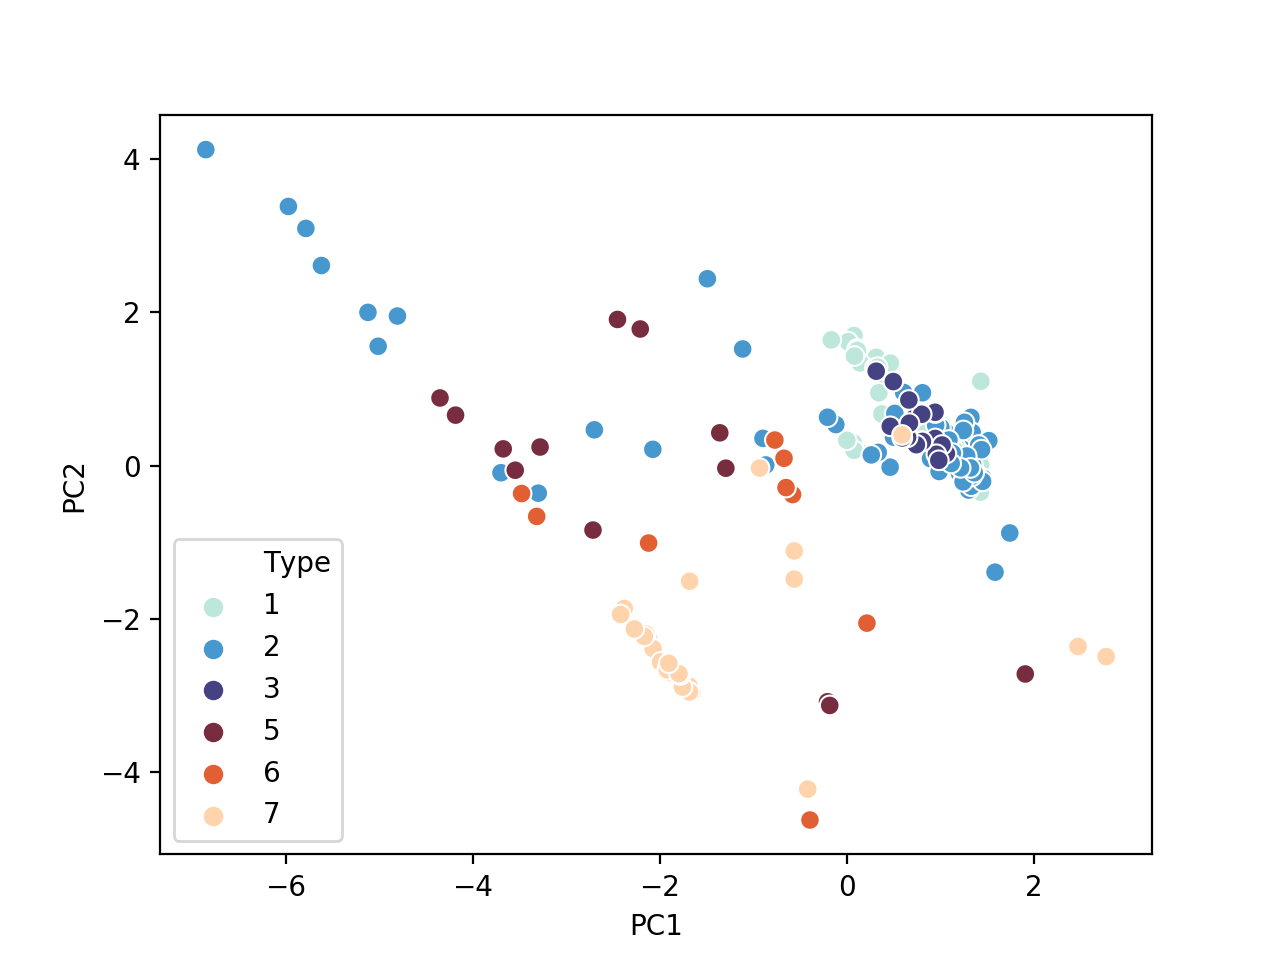
\includegraphics[width=0.7\linewidth]{{fig/e3.4_1}.png}
\end{figure}

I guess we may say the first two principle components perform pretty well on \ilc{Type 7} glass, but not much the others, especially between \ilc{Type 1, 2, 3}, a zoom in plot will look like this:

\begin{figure}[H]
    \centering
    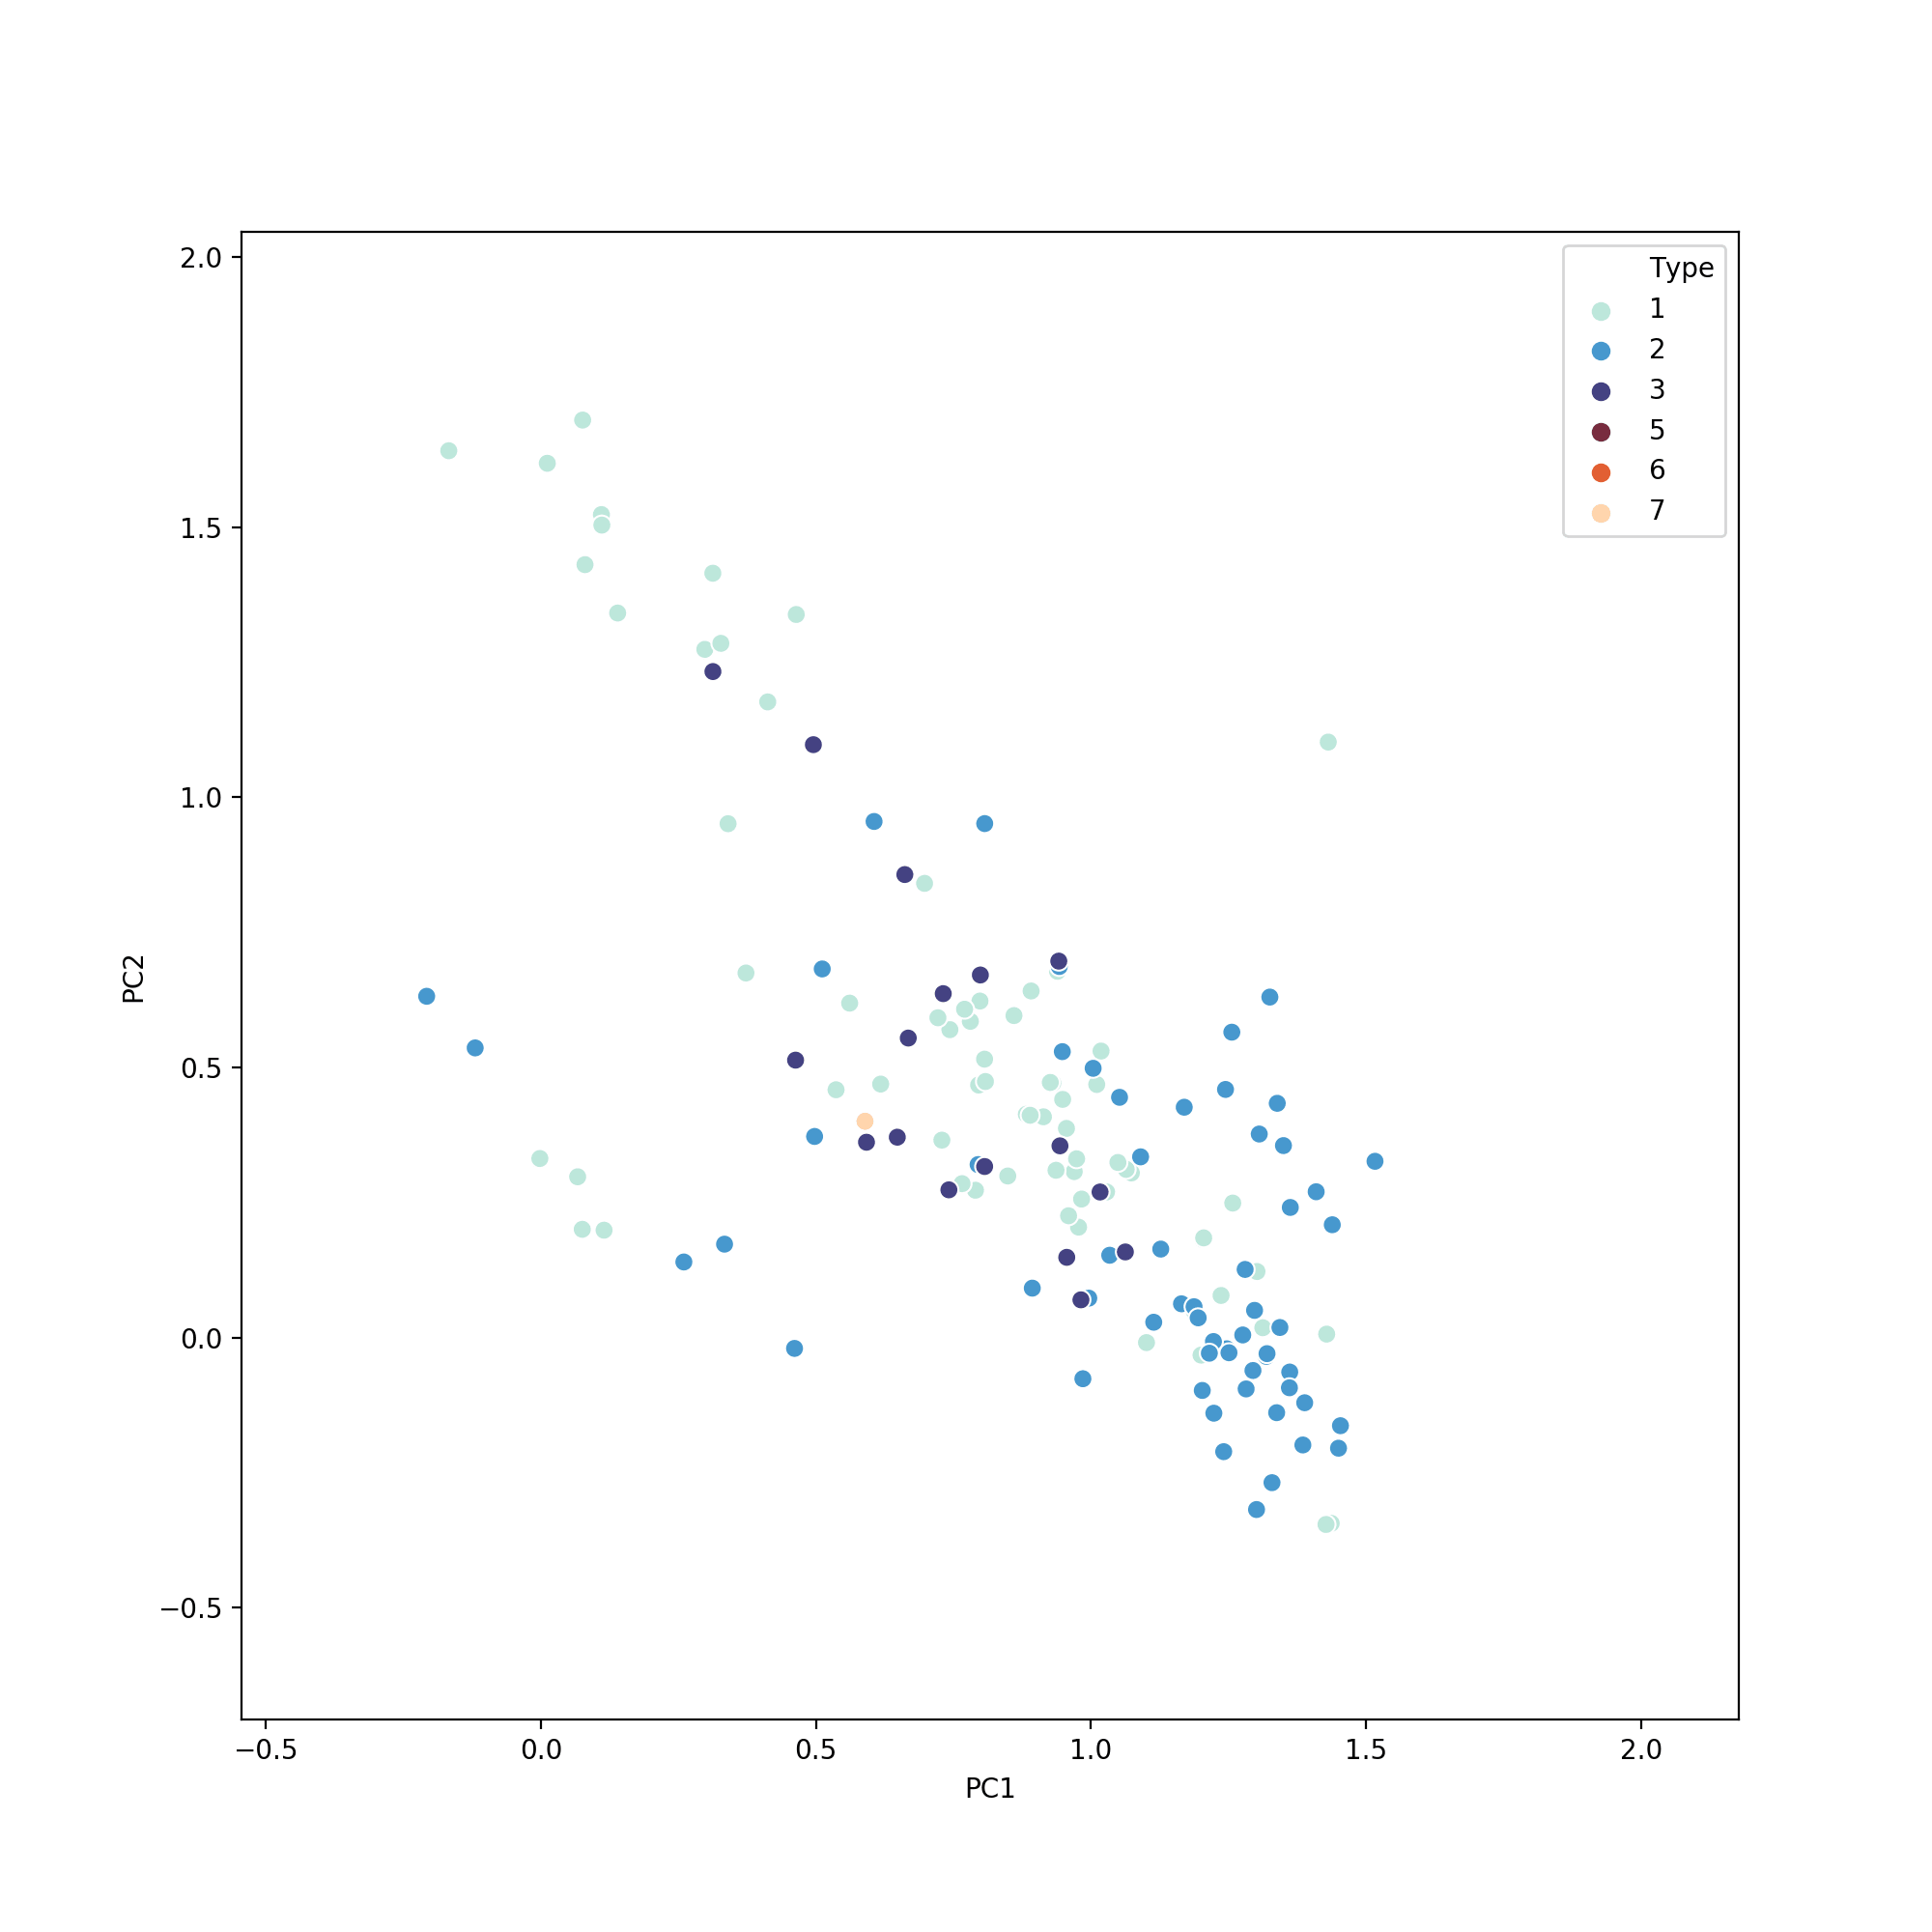
\includegraphics[width=0.5\linewidth]{{fig/e3.4_2}.png}
\end{figure}

This is something rather expected as we have 7 output labels (in fact, 6 output labels as we have no \ilc{Type 4}), but only 2 dimensions to project the clustering. The performance is further limited due to the unbalanced nature of having significantly more \ilc{Type 1} and \ilc{Type 2} samples, granting \ilc{Type 1\&2} glasses to display more features that are potentially similar to other types of glasses (just like doing multiple testing).




\section*{E4. Gaussian Mixture Models }

\section*{Exploration: t-SNE}

\subsection*{Motivation}

% https://www.youtube.com/watch?v=NEaUSP4YerM
% https://medium.com/@violante.andre/an-introduction-to-t-sne-with-python-example-47e6ae7dc58f

There are many dimensionality reduction algorithms, as we have learned in this class, PCA is a dimensionality reduction algorithm that works fairly well on linear datasets and it is known to be used in combination with distance-based clustering algorithms. Intuitively, this makes PCA unapplicable of capturing dataset with non-linear structure -- such as a manifold ``Swiss roll'' we showed in class.

\begin{figure}[H]
    \centering
    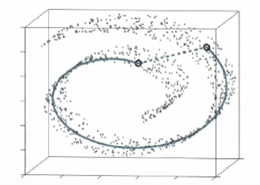
\includegraphics[width=0.4\linewidth]{{fig/exp_swiss_roll}.png}
\end{figure}

Well there are certainly PCA-based algorithms that are designed to handle this problem, e.g., the various avalivable and kernel PCAs, the SNEs and t-SNE in particular attracted my attention as it is a dimensionality reduction algorithm that doesn't wotk with distance-based clustering algorithms, yet yields promising results (\href{https://stats.stackexchange.com/questions/340175/why-is-t-sne-not-used-as-a-dimensionality-reduction-technique-for-clustering-or}{ref.}):



\begin{figure}[H]
\minipage{0.5\textwidth}
  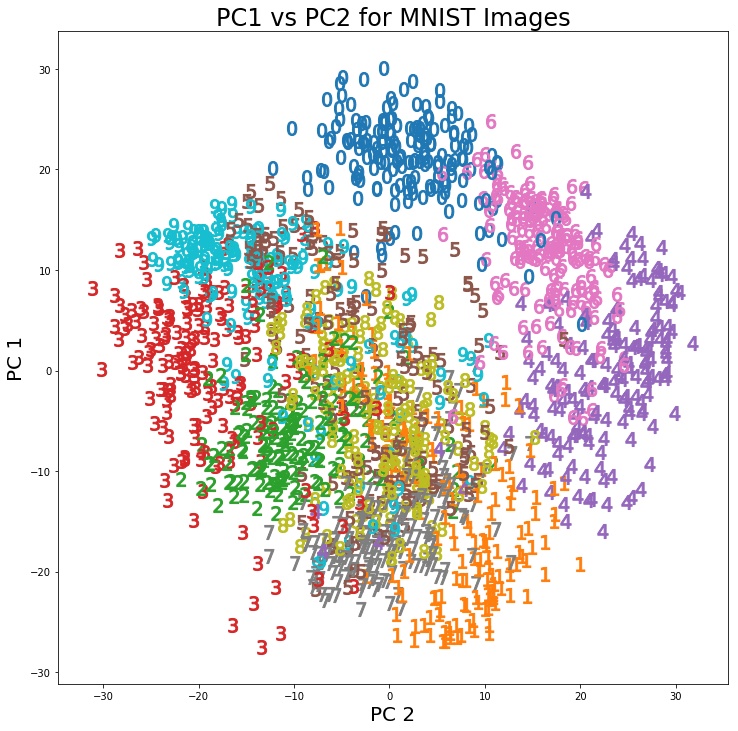
\includegraphics[width=\linewidth]{{fig/exp_pca_minist}.png}
\endminipage\hfill
\minipage{0.5\textwidth}
    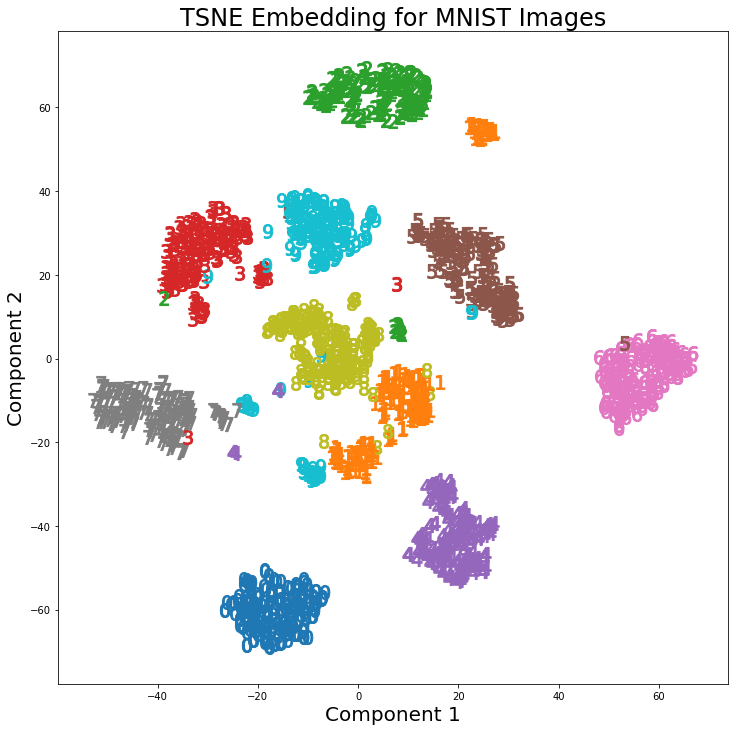
\includegraphics[width=\linewidth]{{fig/exp_tsne_minist}.png}
\endminipage
\end{figure}

Clearly the t-SNE algorithms shows better clusters in comparison to PCA. So in this exploration I will give a brief walk-through on how t-SNE works, run it on the same dataset I used in \textbf{Exercise 3} and interpret the result, then discuss about the advantages between t-SNE and PCA in terms of determinability, locality, usability in combination with clustering algorithms, computational costs, etc.\newline

\subsection*{Mechanism of t-SNE}

As we already familiar from learning PCA, any direct projection of high-dimensional datapoints to lower dimensions will likely result in a mishmash:

\begin{figure}[H]
    \centering
    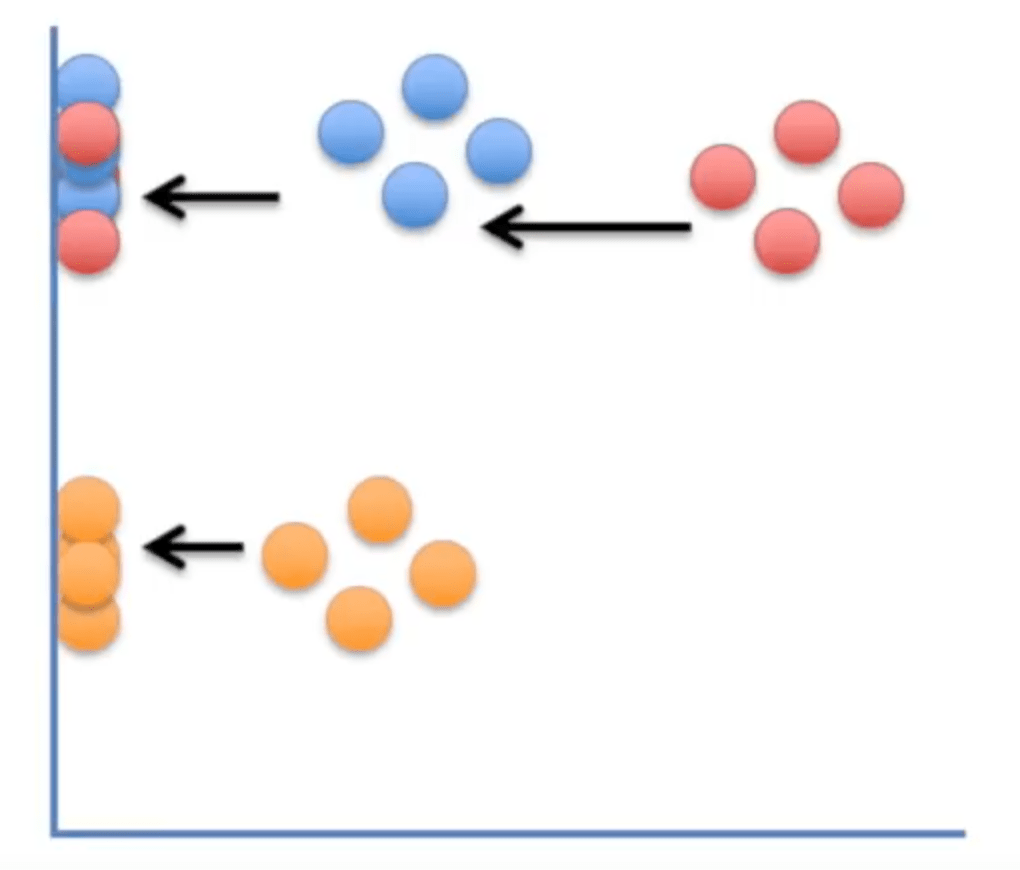
\includegraphics[width=0.4\linewidth]{{fig/exp_direct_pj}.png}
\end{figure}

Intuitively, we would like to move around these projected datapoints, so that there can be a distinguishiable distance between different labels. However, the question is how? Which point should we move? And in which direction? Assume we have the following raw projection of two dimensional data onto one line:


\begin{figure}[H]
    \centering
    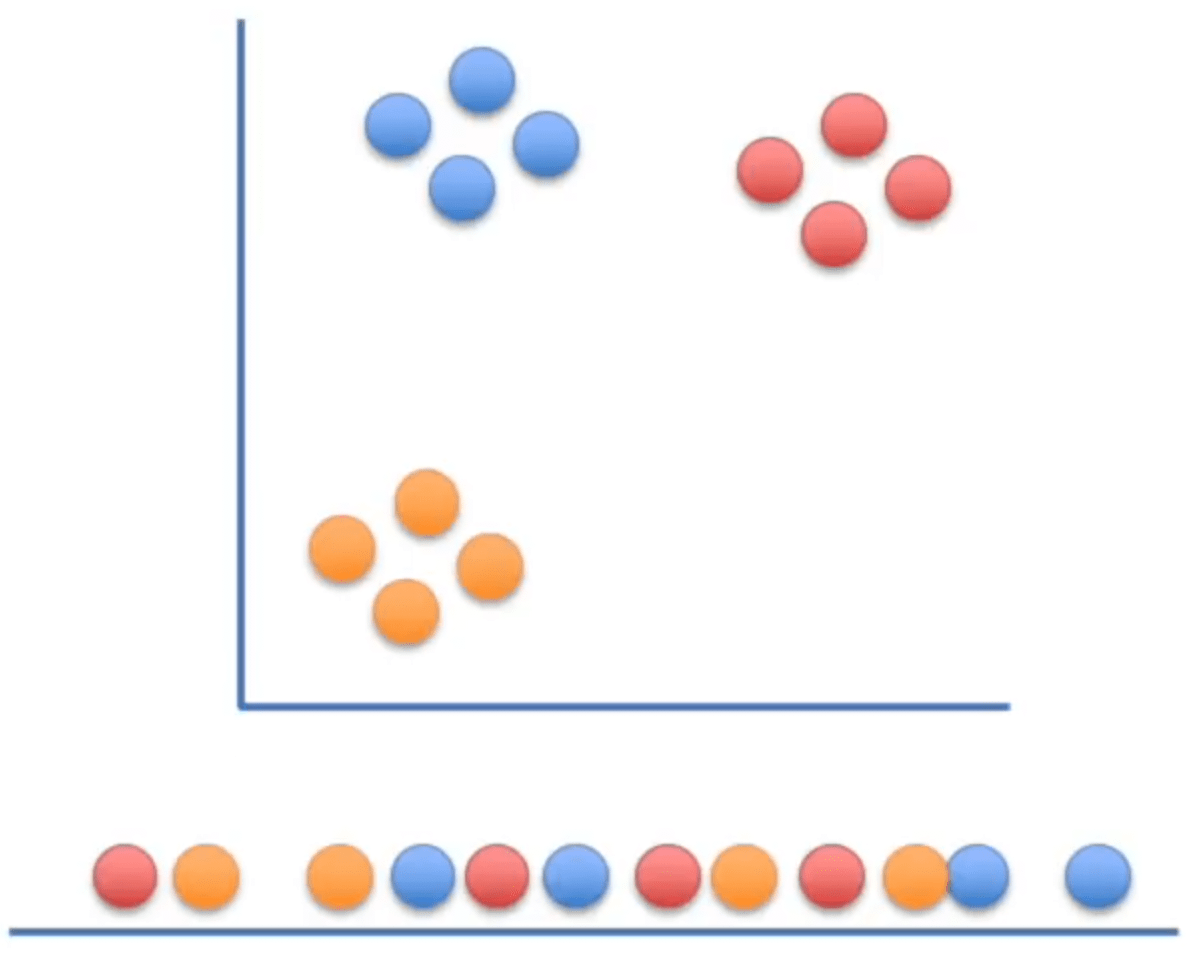
\includegraphics[width=0.5\linewidth]{{fig/exp_tsne_raw}.png}
\end{figure}

t-SNE runs in an iterative manner, as it will move one point at a time untill it reaches the stopping criteria (which is usually numbers of iterations). W.L.O.G., let's check out how will t-SNE move the \textcolor{red}{leftmost red} point:

\begin{enumerate}
    \item First t-SNE will datapoints which is similar to this \textcolor{red}{leftmost red}, which are other \textcolor{red}{red} datapoints.
    \item So naturally, we should move this \textcolor{red}{leftmost red} datapoint closer to other \textcolor{red}{red} datapoints -- which is to its right.
    \item Similarily, since this \textcolor{red}{leftmost red} is far away from the \textcolor{orange}{orange} and \textcolor{blue}{blue} datapoints in its original space, it will like to move away from them -- which is to its left.
\end{enumerate}

So we have the following ``tractions'':
\begin{figure}[H]
    \centering
    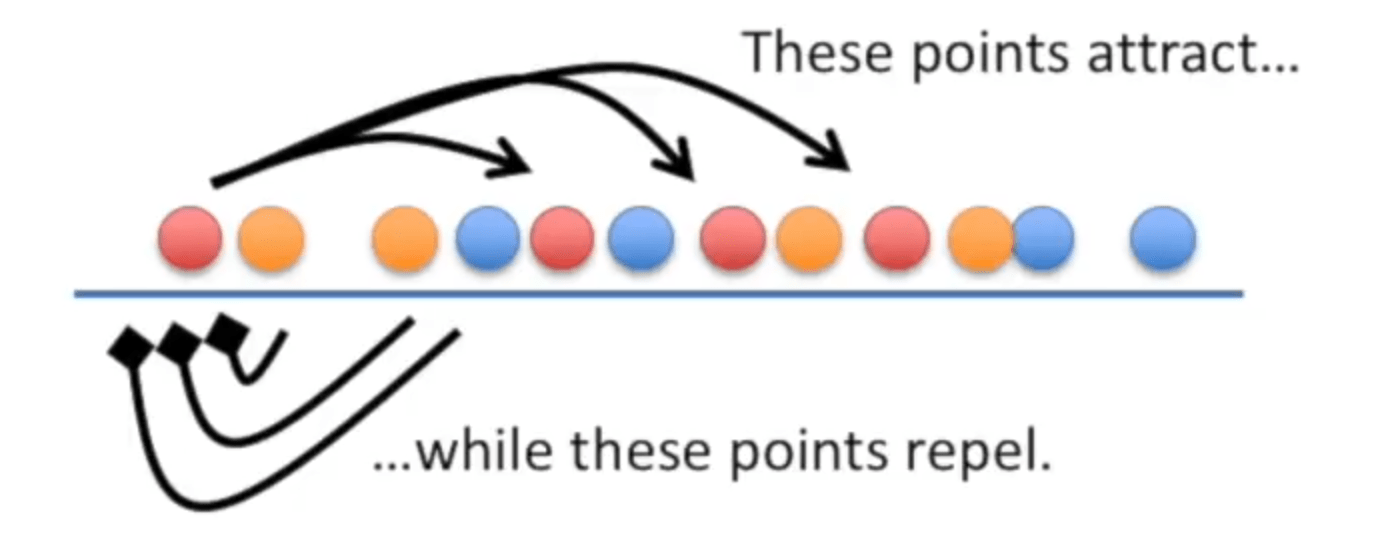
\includegraphics[width=0.5\linewidth]{{fig/exp_tsne_demo}.png}
\end{figure}

Let's assume this time the traction from the \textcolor{red}{red} points are stronger, so the \textcolor{red}{leftmost red} moves to its right for a bit. Then we do this evaluation to each and every points, over and over, untill the stopping criteria is reached, and we may have some nice clusters on this one dimensionl line.\newline

So how does t-SNE determine the similarity between datapoints? It does it, again, in an iterative manner. t-SNE will locate a point first (in this case, it will be the \textbf{black}{black} point from the \textbf{blue}{blue} cluster), and model its relative distances to all other datapoints under a normal distribution curve. So datapoints with same or similar lable, will have a higher probablity score, as it is closer to the center of the normal curve; yet datapoints that is vast unlike to eachother will have a lower probablity score, as it will be at the tails of normal curve.

\begin{figure}[H]
\minipage{0.3\textwidth}
  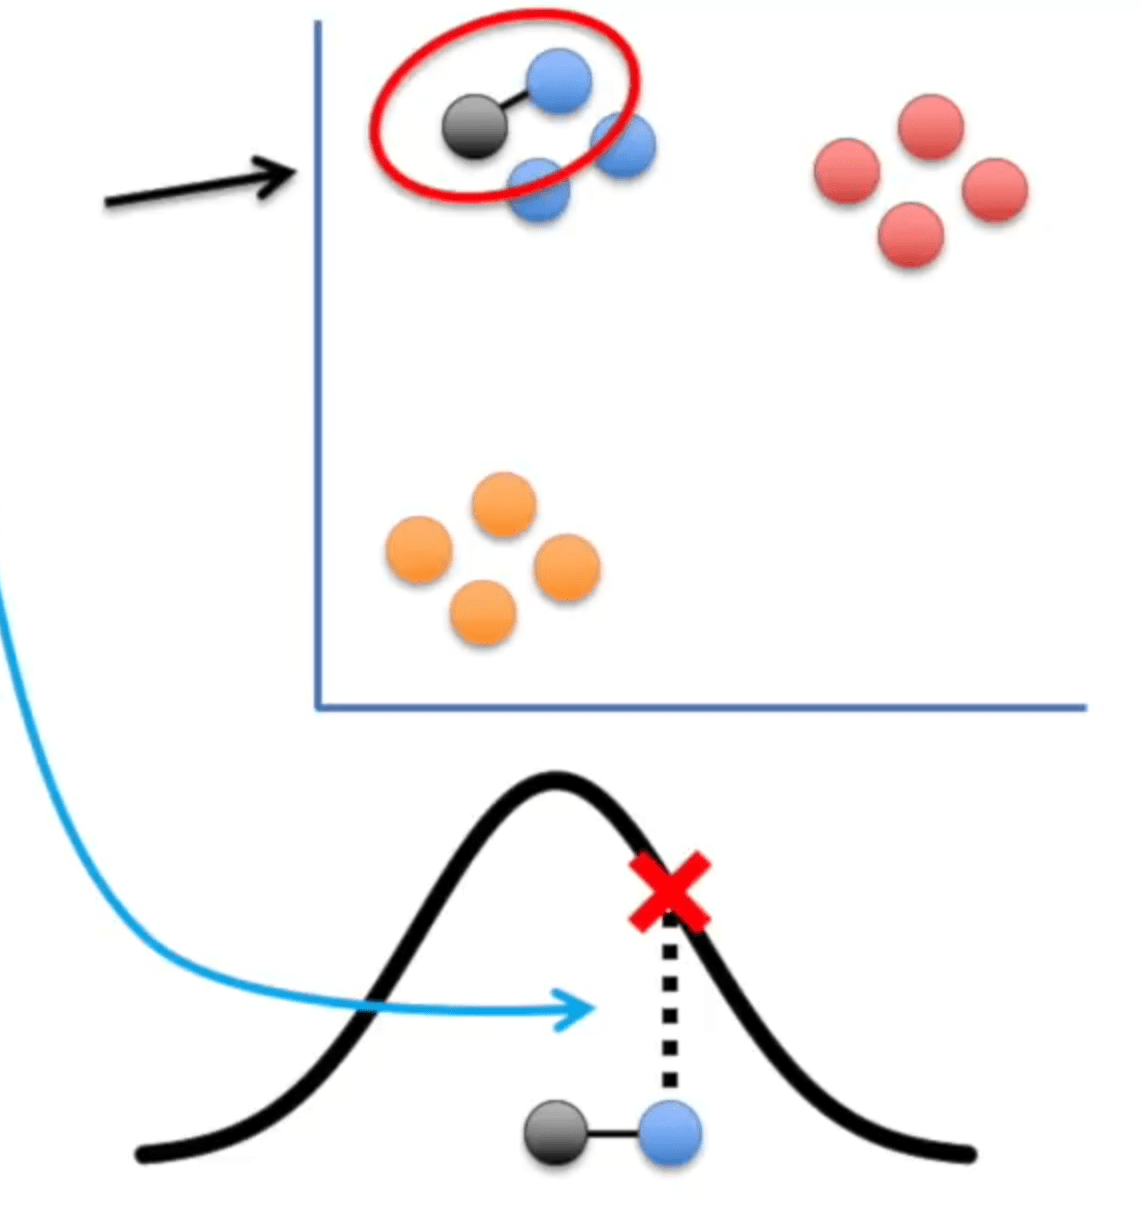
\includegraphics[width=\linewidth]{{fig/exp_tsne_step1.1}.png}
\endminipage\hfill
\minipage{0.3\textwidth}
  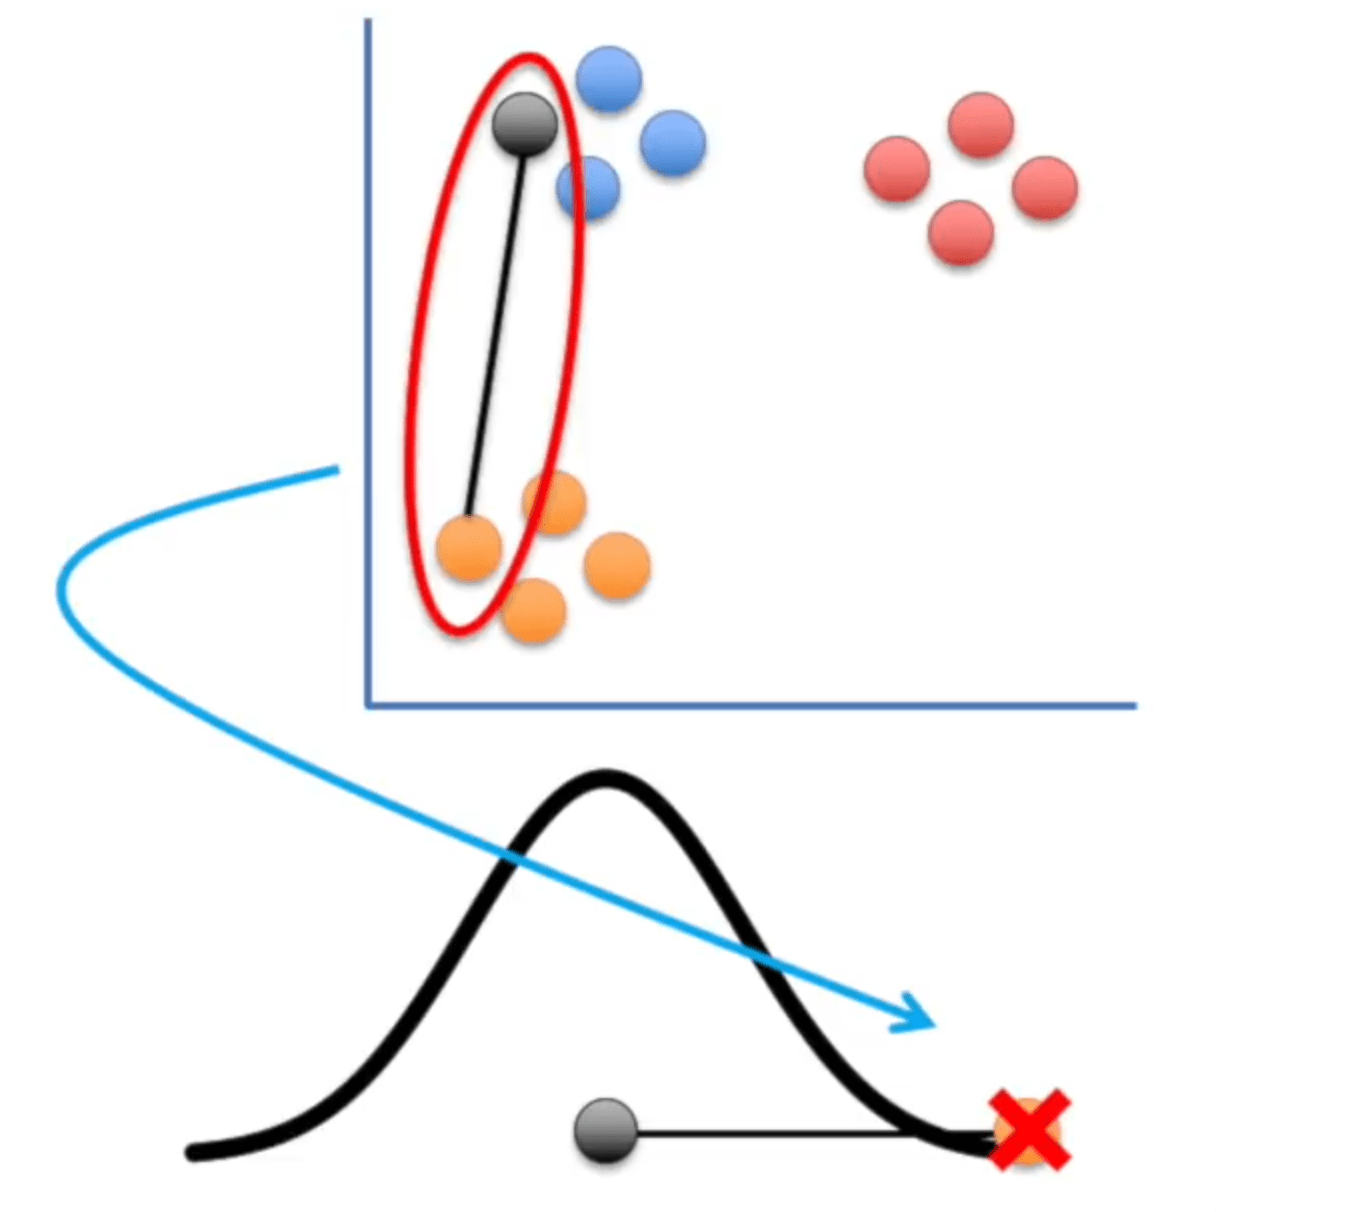
\includegraphics[width=\linewidth]{{fig/exp_tsne_step1.2}.png}
\endminipage\hfill
\minipage{0.3\textwidth}
    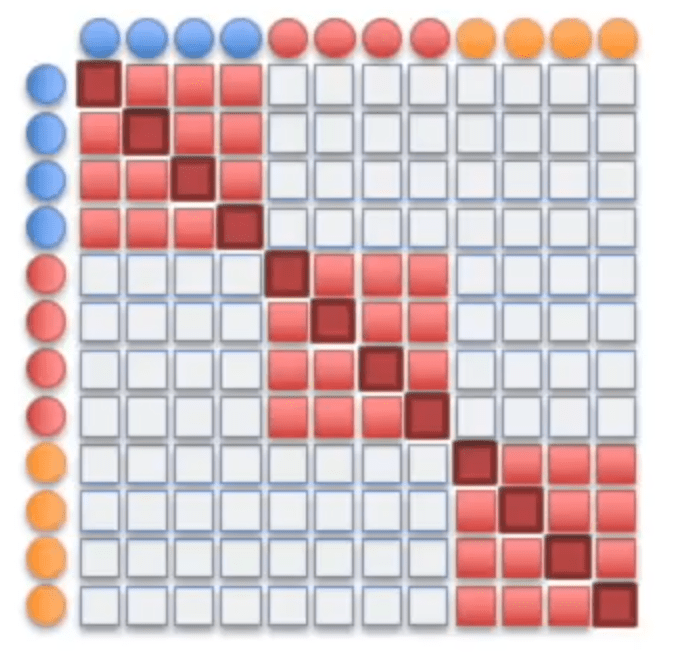
\includegraphics[width=\linewidth]{{fig/exp_tsne_step1.3}.png}
\endminipage
\end{figure}

t-SNE will then ``scale'' these probablity scores to unsure the total probably will be added to 1. In other words, assume datapoint $A$ has relative probablity scores of $p(A_x), p(A_y), \dots p(A_n)$ to datapoint $X, Y, \dots, N$, we will have $p(A_i') = \frac{p(A_i)}{\sum\limits_{j}^{n} p(A_j)}$. Following this procedure, t-SNE will obtain the relative normalized probablity score between every two datapoints, and thus fill this similarity matrix (note that it is common that $p(A_b') \neq p(B_a')$ as datapoints $A, B$ are under two different normal distributions. So t-SNE simple take the average out of these two) -- and the end result will be the rightmost matrix above; where \textcolor{red}{red entries} represent higher similarity.\newline

Now we repeat such matrix filling operation with respect to the one-dimensional line, as we will fill in another matrix where the noralized probablity score will be determined by the relative distance between one point to another on this one-dimensional line. However, instead of modeling its with normal distribution, it will use t-distribution (and therefore, the ``t'' of ``t-SNE'') -- this is because t-distribution curve has a lower center and higher tails in comparison to normal distribution, thus encourges more seperation of datapoints.


\begin{figure}[H]
\minipage{0.7\textwidth}
  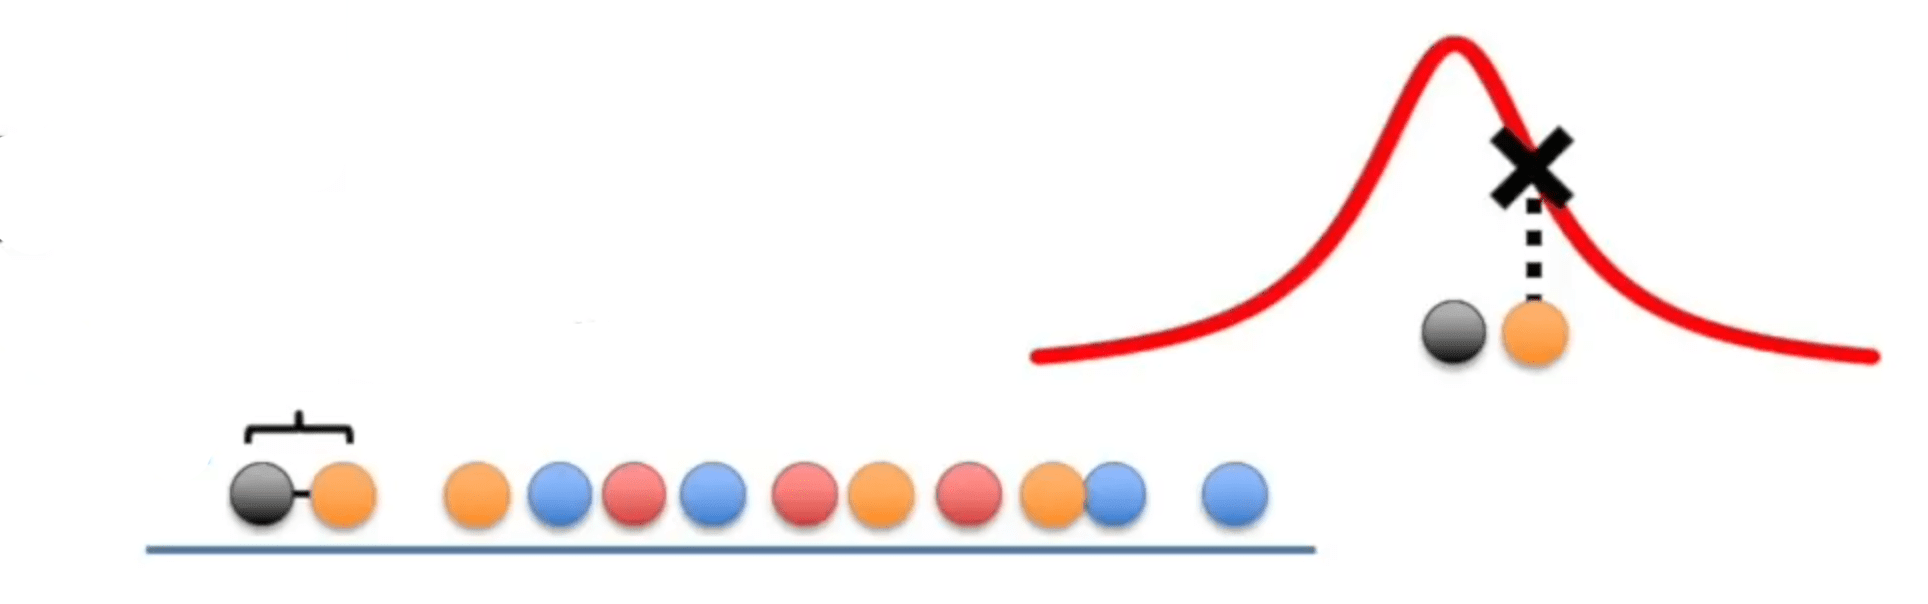
\includegraphics[width=\linewidth]{{fig/exp_tsne_step2.1}.png}
\endminipage\hfill
\minipage{0.3\textwidth}
    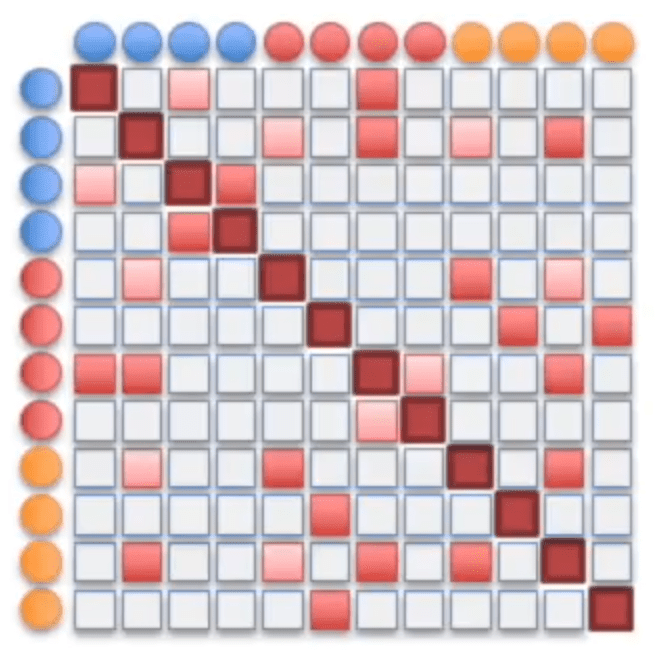
\includegraphics[width=\linewidth]{{fig/exp_tsne_step2.2}.png}
\endminipage
\end{figure}

With the two similarity matrices, t-SNE may then try to ``convert'' the second matrix more like the first one -- and the steps of this conversion will determine the moving direction of each datapoints.

\subsection*{t-SNE on UCI ML Glass Classification Dataset}

I have implemented t-SNE on the UCI ML Glass Classification Dataset I used in \textbf{Exercise 3} and got the following result:

\begin{figure}[H]
\minipage{0.5\textwidth}
  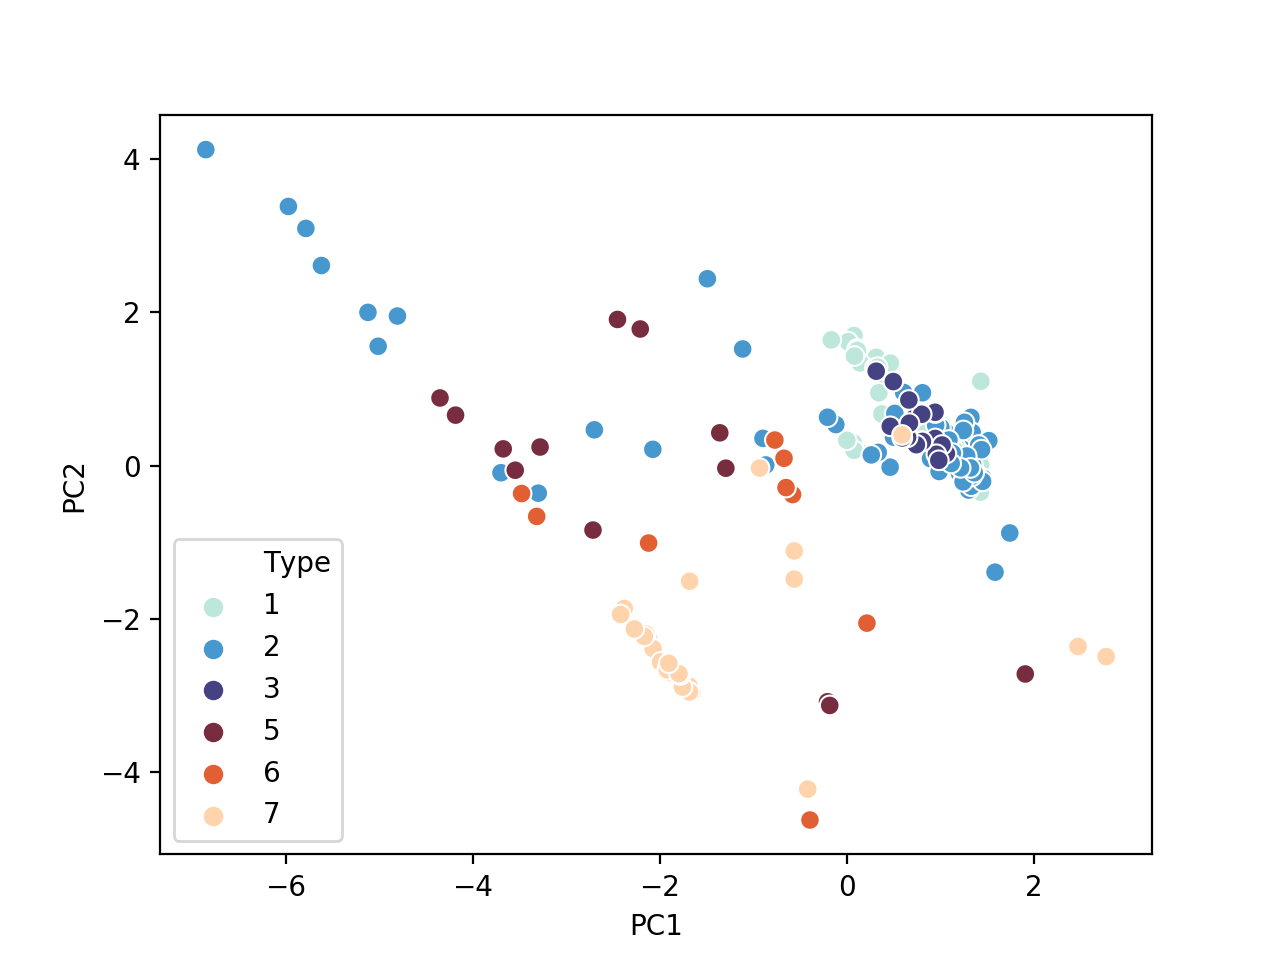
\includegraphics[width=\linewidth]{{fig/e3.4_1}.png}
  \caption*{PCA}
\endminipage\hfill
\minipage{0.5\textwidth}
    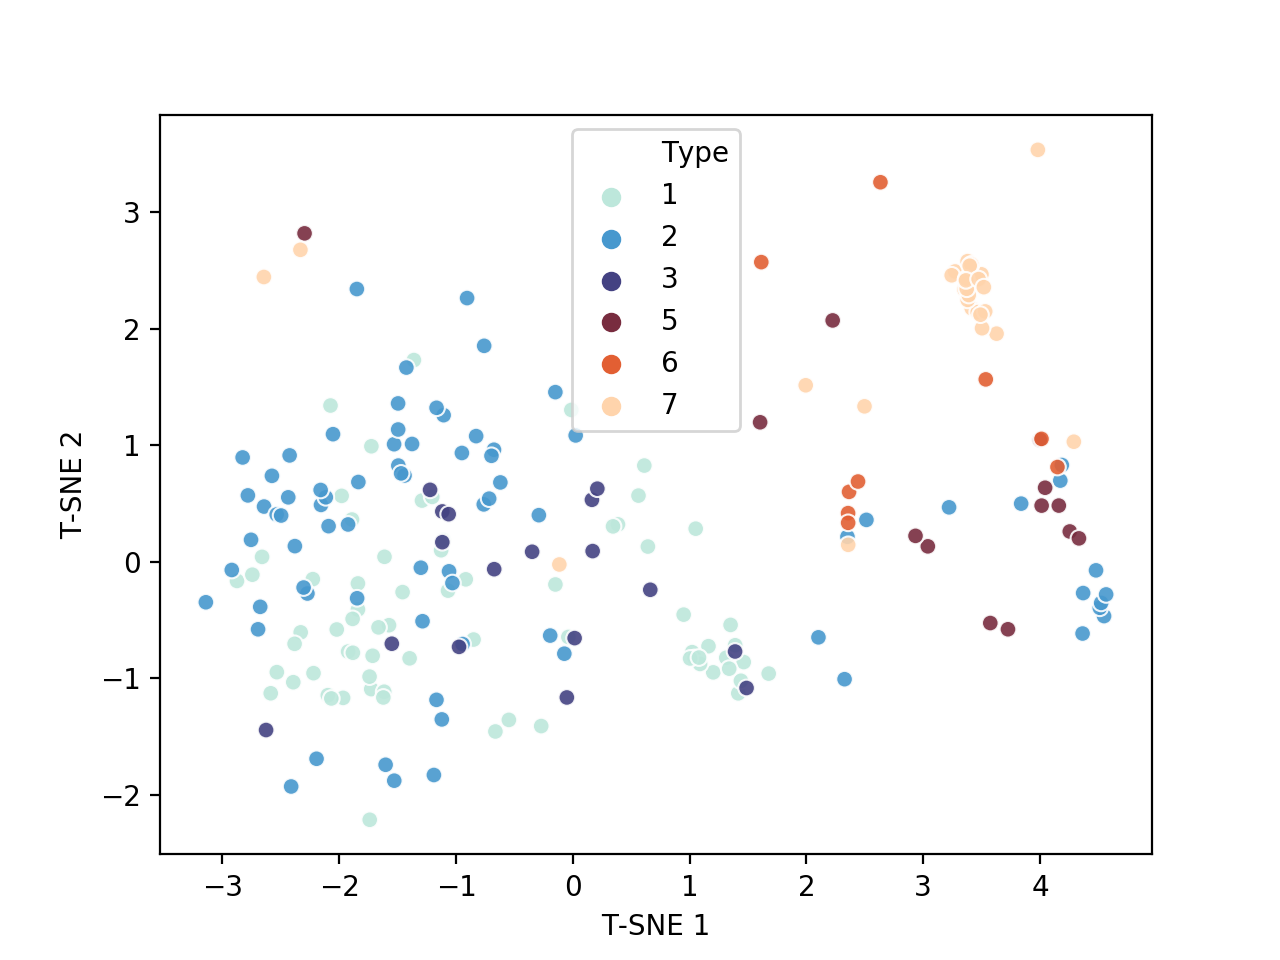
\includegraphics[width=\linewidth]{{fig/exp_glass}.png}
    \caption*{t-SNE}
\endminipage
\end{figure}

Although we don't have a clean clustered result like t-SNE on \ilc{MINIST} did. It is observable that we have better clustering result as the \ilc{Type 5, Type 6, Type 7} glasses are better gathered. Although we still can't effectively distinguish \ilc{Type 1} from \ilc{Type 2} glasses, they are certainly more scattered.

(please refer to \ilc{A4/code/exploration} for code implementation.)

\subsection*{t-SNE vs PCA}

Although t-SNE offers better clustering visualization on many popular tasks, it also has its pros and cons. The main pros, are that t-SNE can certainly able to capture manifold structure, and it is better on visualization due to the procedure of t-SNE encourages different datapoints to ``move away from eachother,'' where PCA only cares about the maximum of sum of squared variance.\newline

t-SNE also has many cons, and one of the most significant one is probably its incompability with distanced-based clustering algorithms. As we are directly moving the datapoints around in a lower-dimensional space, these datapoints lose their original distance relationship and thus become incapable of being a direct feed of distance-based clustering algorithms. Also on this note, t-SNE is not capable of learning a high-dimensional space to a lower-dimensions, but rather just lower the dimensions of known data -- so if an unseen data joins, it can't directly project it onto a lower-dimensionl space.\newline

Further t-SNE is a non-determistic algorithm as it has a turnable paramater \textit{perplexity}, which is a loose balancer between the local and global aspect of given data, so you might have to run multiple trials to achive the optimal result. This is especially a problem as t-SNE is a lot more computational intense than PCA due to 1) it has to calculate the similarity scores that is proporsional to the combinations of datapoints, but not simply project all datapoints on to a line; 2) it has to do it iteraively over and over.

The effect of this parameter is complicate, but according to \href{https://distill.pub/2016/misread-tsne/}{many articles} it works best if it is a rough estimation of cluster size. This implies t-SNE is probably not so suitable to unbalanced dataset (like the UCI ML Glass Classification I used). PCA, on the other hand, is parameter-free, but I don't consider this to be such a major advantage as the countless kernel PCA algorithms has much more turnable parameters.\newline

A more through discussion between t-SNE and PCA can be found \href{https://stats.stackexchange.com/questions/238538/are-there-cases-where-pca-is-more-suitable-than-t-sne}{here} and \href{https://stats.stackexchange.com/questions/263539/clustering-on-the-output-of-t-sne}{here}.

\end{document}

